
\documentclass[10pt, openany]{book}

\usepackage{../preamble}
\addbibresource{../ref.bib}
\AtEveryBibitem{\clearfield{note}}

\fancyhead[LE,RO]{\thepage}
\fancyhead[RE]{\textbf{Copilot}}
\fancyhead[LO]{\textit{开发手册}}

\begin{document}

\frontmatter

\title{\textbf{Coplilot}\\ \large 开发手册 }
\author{Lao Chen}
\date{\today}
\maketitle
\tableofcontents

\mainmatter

\chapter*{前言}
\phantomsection
\addcontentsline{toc}{chapter}{前言}

本手册记录 AI 辅助编程系统 Copilot 的设计思路与实践经验。
核心问题是：\textbf{大语言模型（LLM）在代码生成中的系统性缺陷如何被约束？}

\begin{itemize}
    \item LLM 生成的代码不可靠——语法错误、类型错误、逻辑错误、幻觉 API~\cite{Chen2021Codex}
    \item 原生 Agent（CodeBuddy）在真实项目中暴露出五类典型事故——走错项目、端口误配、虚假信息信任、PID 误杀、规则膨胀
    \item 提示词工程有无法逾越的天花板~\cite{Liu2023LostInMiddle}——必须引入编译器、类型系统、权限控制等\textbf{外部约束}
\end{itemize}

本手册分为七章：
\begin{enumerate}
    \item LLM 与 Transformer——从统计语言模型到大语言模型的理论脉络
    \item 复盘——CodeBuddy 原生实践中的 LLM Agent 失控
    \item 架构约束——全栈架构如何缩减 LLM 的可能输出空间
    \item 编译器约束——类型系统是自然语言的形式化离散化
    \item JCS 保护约束——确定性代码生成的边界
    \item Copilot 设计规范——五层拦截器架构
    \item 技术实施方案——开发语言选型、AIO 界面嵌入、部署路线
\end{enumerate}

% ================================================================
\chapter{LLM 与 Transformer 概述}
% ================================================================

\section{从神经语言模型到 Transformer}

大语言模型（LLM）的本质是\emph{统计语言模型}：给定前文，
预测下一个 token 的条件概率分布。
其理论基础可追溯到 Bengio 等提出的\emph{神经概率语言模型}~\cite{Bengio2003NNLM}——
用多层感知机学习词的分布式表示（word embedding），
将离散的词汇映射到连续的向量空间中~\cite{Mikolov2013Word2Vec}。

在此之后的十年间，序列建模的主流架构是循环神经网络（RNN）及其变体：
LSTM~\cite{Hochreiter1997LSTM} 用门控机制缓解梯度消失，
GRU~\cite{Cho2014GRU} 简化为更新门+重置门。
Seq2Seq 框架~\cite{Sutskever2014Seq2Seq} 引入编码器-解码器结构，
Bahdanau 等进一步提出注意力机制~\cite{Bahdanau2015Attention}——
让解码器在生成每个输出时动态地关注编码器的不同位置，
这是 Transformer 架构中自注意力机制的直接前身。

\section{Transformer 架构}

Vaswani 等在 2017 年提出 Transformer 架构~\cite{Vaswani2017Attention}，
彻底抛弃了循环结构，代之以\emph{自注意力机制（Self-Attention）}：

\begin{definition}[缩放点积注意力]
给定查询 \(Q\)、键 \(K\)、值 \(V\)，
\[
\text{Attention}(Q,K,V) = \text{softmax}\!\left(\frac{QK^\top}{\sqrt{d_k}}\right) V
\]
其中 \(d_k\) 是键向量的维度，除以 \(\sqrt{d_k}\) 防止内积过大导致 softmax 梯度消失。
\end{definition}

\noindent Transformer 的核心创新：
\begin{enumerate}
    \item \textbf{多头注意力（Multi-Head Attention）}：并行运行 \(h\) 个注意力头，
        每个头在不同的投影子空间中学习不同的关联模式~\cite{Vaswani2017Attention}
    \item \textbf{位置编码（Positional Encoding）}：由于没有循环结构，
        Transformer 通过正弦/余弦函数或可学习的位置嵌入注入序列顺序信息。
    \item \textbf{残差连接 + 层归一化}：每个子层（自注意力/前馈网络）的输出都经过残差连接和层归一化，
        保证深层网络的可训练性~\cite{Vaswani2017Attention}。
    \item \textbf{编码器-解码器 vs 解码器仅}：原始 Transformer 使用编码器-解码器结构；
        但 GPT 系列~\cite{Radford2018GPT,Radford2019GPT2,Brown2020LanguageModels} 仅使用解码器（单向自注意力），
        在自回归语言建模（预测下一个 token）上效果更好。
\end{enumerate}

自注意力机制的复杂度为 \(O(n^2 \cdot d)\)（\(n\) 是序列长度，\(d\) 是维度），
这是 Transformer 的核心计算瓶颈。
后续工作如 Transformer-XL~\cite{Dai2019TransformerXL} 引入段级递归和相对位置编码，
突破了固定上下文长度的限制。

\section{预训练时代：BERT、GPT、T5}

2018--2020 年，预训练-微调（Pre-train + Fine-tune）范式彻底改变了 NLP：

\begin{itemize}
    \item \textbf{GPT（自回归语言模型）}：Radford 等~\cite{Radford2018GPT} 提出生成式预训练——在大量无标注文本上训练一个单向 Transformer 解码器，预测下一个 token；然后在下游任务上微调。GPT-2~\cite{Radford2019GPT2} 证明，仅用语言建模目标训练的 1.5B 参数模型即可在多个 NLP 任务上实现 zero-shot 迁移
    \item \textbf{BERT（自编码语言模型）}：Devlin 等~\cite{Devlin2019BERT} 提出掩码语言模型（MLM）——随机遮蔽 15\% 的输入 token，让模型从双向上下文中预测被遮蔽的词。配合下一句预测（NSP）任务，BERT 在 11 项 NLP 基准上刷新了记录。\textbf{关键区别}：GPT 单向 → 适合生成；BERT 双向 → 适合理解
    \item \textbf{T5（统一框架）}：Raffel 等~\cite{Raffel2020T5} 将所有 NLP 任务统一为 Text-to-Text 格式——输入是文本，输出也是文本。翻译、问答、摘要、分类全部用同一架构处理。T5 的最重要贡献是系统的预训练目标对比实验
\end{itemize}

这段时期确立了三个核心思想，至今仍是 LLM 的基础~\cite{Brown2020LanguageModels,Devlin2019BERT,Raffel2020T5}：
(1) 更大规模 = 更好性能，(2) 自监督预训练可替代人工标注，
(3) Transformer 是通用序列建模架构。

\section{规模化定律}

Kaplan 等~\cite{Kaplan2020Scaling} 系统研究了\emph{神经网络语言模型的缩放定律（Scaling Laws）}：
测试损失 \(L\) 与模型参数量 \(N\)、训练数据量 \(D\)、训练计算量 \(C\) 之间遵循幂律关系：
\[
L(N) = \left(\frac{N_c}{N}\right)^{\alpha_N},\quad
L(D) = \left(\frac{D_c}{D}\right)^{\alpha_D},\quad
L(C) = \left(\frac{C_c}{C}\right)^{\alpha_C}
\]

这个发现直接催生了 GPT-3~\cite{Brown2020LanguageModels}——175B 参数，训练于 570GB 文本，
展现出\emph{上下文学习（In-Context Learning）}能力：无需微调，仅通过提示词中的少量示例即可完成新任务。

\noindent \textbf{关键发展脉络}：
\begin{itemize}
    \item \textbf{Chinchilla 修正}：Hoffmann 等~\cite{Hoffmann2022Chinchilla} 发现 Kaplan 的定律低估了数据的重要性——\textbf{给定计算预算，模型参数和训练 token 数应等比增长}。70B 参数的 Chinchilla 用 1.4T tokens 训练，性能超过 280B 参数的 Gopher
    \item \textbf{涌现能力}：Wei 等~\cite{Wei2022Emergent} 系统记录了大模型的\emph{涌现能力（Emergent Abilities）}——当模型规模超过某个临界值时，之前不存在的思维链推理、指令遵循、多步算术等能力突然出现。这解释了为什么 BERT（340M）没有 GPT-3（175B）那样的通用能力
    \item \textbf{PaLM}：Chowdhery 等~\cite{Chowdhery2022PaLM} 将模型规模推到 540B 参数，展示了~\emph{思维链提示（Chain-of-Thought）}~\cite{Wei2022ChainOfThought} 下的多步推理突破——在数学推理基准 GSM8K 上接近人类水平
    \item \textbf{LLaMA}：Touvron 等~\cite{Touvron2023LLaMA} 证明\emph{仅用公开数据}即可训练出有竞争力的 LLM，开启了开源 LLM 的浪潮
\end{itemize}

\section{对齐：RLHF 与指令微调}

规模化带来了能力，也带来了不可控性。
GPT-3 可以生成流畅的文本，但不一定遵循用户意图——
可能产生有害内容、编造事实（幻觉）、或忽视指令约束~\cite{OpenAI2023GPT4,Kadavath2022SelfEvaluation}。

Ouyang 等~\cite{Ouyang2022InstructGPT} 提出了\emph{基于人类反馈的强化学习（RLHF）}：
\begin{enumerate}
    \item \textbf{监督微调（SFT）}：用人类标注的高质量指令-回复对微调预训练模型
    \item \textbf{奖励模型（RM）}：收集同一提示下的多个模型输出，由人类排序，训练一个奖励模型来预测人类偏好
    \item \textbf{PPO 强化学习}：用奖励模型作为奖赏信号，通过 PPO 算法进一步优化策略
\end{enumerate}
1.3B 参数的 InstructGPT 就能在人类偏好评测中超过 175B 的 GPT-3，
证明了\emph{对齐比规模更重要的原则}~\cite{Ouyang2022InstructGPT}。

GPT-4~\cite{OpenAI2023GPT4,Achiam2025GPT4System} 进一步将 RLHF 扩展到多模态（文本+图像），
在统一律师资格考试（Bar Exam）中排名前 10\%，
且通过红队测试和系统级安全措施大幅降低有害输出~\cite{OpenAI2023GPT4}。

\noindent \textbf{对齐的局限}：RLHF 提升了指令遵循能力，但无法消除\emph{幻觉}——
LLM 仍可能自信地生成看似合理但完全错误的内容~\cite{Kadavath2022SelfEvaluation}。
这一缺陷是 Copilot 编译器反馈循环的\emph{根本动机}：
人类使用 LLM 不是为了得到``可能正确的答案''，而是需要\textbf{经验证正确的代码}。

\section{代码生成 LLM}

LLM 在代码生成领域的突破始于 Codex~\cite{Chen2021Codex}——
一个基于 GPT-3 微调的代码专用模型，训练于 GitHub 公共仓库的 159GB Python 文件。
Codex 在 HumanEval 基准上实现了 28.8\% 的 pass@1 准确率
（GPT-3 仅 0\%），证明了\emph{领域特化训练}的有效性。

\noindent 后续发展：
\begin{itemize}
    \item \textbf{StarCoder}~\cite{Li2022StarCoder}：在 The Stack（6.4TB 开源代码，358 种编程语言）上训练的 15.5B 参数模型，采用 Multi-Query Attention 减少推理开销
    \item \textbf{GPT-4}~\cite{OpenAI2023GPT4}：通用模型的代码能力大幅提升，在 HumanEval 上达到 67\%（零样本）和 88\%（结合自我修复）
    \item \textbf{Austin 等}~\cite{Austin2021Program} 系统评估了 LLM 在程序合成中的表现，发现\emph{即使最强的模型在生成完整程序时仍有约 40\% 的错误率}
\end{itemize}

代码生成 LLM 的\emph{根本局限}与本手册的核心论点直接相关~\cite{Chen2021Codex}：
\textbf{LLM 生成的是统计概率最高的 token 序列，而非类型安全的程序。}
它不理解类型系统~\cite{Pierce2002TAPL}、
无法保证跨文件一致性、
不能验证 API 的真实存在性。
这些正是编译器、类型系统和架构约束需要填补的空白。

\section{Agent 范式}

LLM 从``被动生成''到``主动执行''的转变，由 Agent 范式驱动：

\begin{itemize}
    \item \textbf{ReAct}~\cite{Yao2023ReAct}：将推理（Reasoning）和行动（Acting）交织在一起——LLM 生成一个\emph{想法}，根据想法调用工具，观察工具返回的结果，再生成下一个想法。ReAct 在知识密集型任务上将幻觉率从 20\% 降到 12\%~\cite{Yao2023ReAct}
    \item \textbf{Reflexion}~\cite{Shinn2024Reflexion}：在 ReAct 的基础上增加了\emph{口头强化学习}——Agent 失败后，将执行轨迹和结果作为``反思''存入记忆，下次执行时利用反思避免重复错误。这直接启发了 Copilot 的编译器反馈循环
    \item \textbf{Self-Refine}~\cite{Wang2023SelfRefine}：LLM 生成初稿后，用自身的反馈进行迭代改进——不需要外部监督信号。在代码优化任务上，Self-Refine 将 pass@1 提升 10--20\%
    \item \textbf{AutoGen}~\cite{Wu2024AutoGen}：多 Agent 协作框架——多个 LLM Agent 通过结构化对话协作完成任务，支持角色分工（编码员/审查员/测试员）、人工介入、代码执行沙箱
\end{itemize}

\begin{principle}[LLM 的理论边界]
LLM 的所有进步——从 Transformer~\cite{Vaswani2017Attention} 到 RLHF~\cite{Ouyang2022InstructGPT} 到 Agent~\cite{Yao2023ReAct}——
都未触及一个根本问题：\textbf{LLM 的输出是概率性的，不是确定性的}。

Scaling Laws~\cite{Kaplan2020Scaling,Hoffmann2022Chinchilla} 说规模越大、性能越好——但\emph{对数收益}。
涌现能力~\cite{Wei2022Emergent} 说更大的模型有新能力——但\emph{不可预测何时出现}。
RLHF 说可以对齐——但\emph{无法消除幻觉}~\cite{Kadavath2022SelfEvaluation}。

\textbf{Copilot 的存在理由，就是为 LLM 的模糊输出提供确定性的外部约束。}
编译器~\cite{Aho2006Compilers} 不会产生幻觉。
类型系统~\cite{Pierce2002TAPL} 不会产生幻觉。
权限白名单不会产生幻觉。
\textbf{这些都是 LLM 所完全欠缺的——本手册要构建的正是这座桥梁。}~\cite{Chen2024RPCFunctor}
\end{principle}

\section{孔洞驱动开发（Hole-driven Development）}

LLM 在面对复杂 F\# 逻辑时，往往因为一次性输出过多而导致类型推断混乱。
模型试图在一次生成中完成整个函数的实现，结果是\emph{概率空间的大跨步跃进}——每一步都可能累积类型错误。

\textbf{解决方案}：引入\emph{孔洞驱动开发}——允许 LLM 在概率不确定时输出占位符：

\begin{lstlisting}[language=FSharp]
// LLM 对某些类型推导不确定时，用孔洞代替
let processUser user =
    let enriched = ??todo_hole  // ← 孔洞：LLM 承认此处不确定
    enriched
\end{lstlisting}

L3 FCS 拦截器捕获 \cmd{??todo\_hole} 位置，提取该上下文的精确类型需求（从 FCS 的类型检查结果中获得该位置的\emph{唯一合法类型}），\textbf{反向注入}给 LLM 作为下一轮的上下文：

\begin{enumerate}
    \item LLM 生成含孔洞的代码 → L3 编译检查 → FCS 返回该孔洞位置的\emph{期望类型}
    \item Copilot 将期望类型格式化为精确的补全指令 → 注入 LLM 提示词
    \item LLM 只填充孔洞（而非重新生成整个函数）→ 第 2 轮编译通过率大幅提升
\end{enumerate}

\begin{principle}[非对称收敛]
    孔洞驱动的本质是\emph{将单次大跨步生成解构为多次小步收敛}。
    LLM 不需要一次性猜对所有类型——只需要在编译器反馈的引导下，
    逐步填补不确定的区域。每一步的搜索空间都远小于上一步。
    
    这是\emph{非对称收敛（Asymmetric Convergence）}：
    搜索空间随进度指数级缩小，而非线性反思中的恒定搜索空间。
\end{principle}

\section{语义空间缩减率的形式化}

在 \S1.6 讨论 JCS 约束时，可以形式化地量化\emph{架构约束对生成空间的影响}：

\begin{definition}[语义空间缩减率]
设 LLM 在无约束条件下的合法代码生成空间为 \(\Omega_{\text{raw}}\)，
在 JCS 约束（\pathref{Design-*.json} 锁定的接口 Functor 映射）下的合法生成空间为
\(\Omega_{\text{JCS}}\)。则：
\[
\text{缩减率}\ \rho = \frac{|\Omega_{\text{JCS}}|}{|\Omega_{\text{raw}}|} \ll 1
\]
\end{definition}

\textbf{直观理解}：
\begin{itemize}
    \item \(\Omega_{\text{raw}}\)：LLM 可以生成任意 F\# 代码——任意函数签名、任意类型定义、任意模块引用。搜索空间 = 无穷大（组合爆炸）
    \item \(\Omega_{\text{JCS}}\)：JCS 锁定 RPC 接口的 Functor 映射后——API 签名的输入/输出类型已由 \pathref{Design-*.json} 确定，函数的\emph{骨架}（管道结构、错误处理模式）已由 ROR 约定固定。LLM 只在\emph{业务逻辑}上有自由度——搜索空间缩小了数个数量级
\end{itemize}

这种\emph{确定性降维打击}的理论依据：
\begin{itemize}
    \item 原生 F\# 的合法代码空间 ≈ 所有可能的 token 序列
    \item JCS 约束后的合法代码空间 ≈ 所有可能的\emph{业务逻辑} token 序列（骨架已确定）
    \item 后者远小于前者——这就是为什么在 JCS 体系下 LLM 的正确率显著提升
\end{itemize}

\begin{principle}[约束即降维]
    每增加一层约束（类型→架构→命名约定→ROR 模式），
    \(\Omega\) 就缩小一个数量级。
    LLM 的正确率与 \(\Omega\) 的大小成\emph{反比}。
    
    这不是``限制 AI 的创造力''——这是\emph{将 AI 从不可能完成的任务
    （在无穷空间中搜索）解放到可能完成的任务（在有限空间中搜索）}。
\end{principle}

% ================================================================
\chapter{复盘：CodeBuddy 原生实践中的 LLM Agent 失控}
% ================================================================

\section{为什么要复盘？}

在讨论理论方案之前，必须先审视\textbf{现实}——
一个真实的 LLM Agent（CodeBuddy）在为期一周的生产级开发中，
暴露出了哪些问题，造成了多大的损失，
以及\textbf{仅靠提示词工程能否解决}这些问题。

本节基于 \pathref{c:/Dev/.codebuddy/log/} 目录下
2026-06-23 至 2026-06-30 的 64 条审计日志，
提炼出五类典型事故。

\section{五大典型事故}

\subsection{走错项目（2026-06-29 21:15）}

\textbf{场景}：用户报告 ``demo 下没看到前端渲染技术菜单''。

\begin{itemize}
    \item \textbf{Agent 行为}：搜索 Aiarwa 项目目录 → 未找到目标文件 →
        \textbf{跳转到 AIO 项目}（桌面应用 AvaloniaApp）→
        排查方向完全错误
    \item \textbf{根因}：Aiarwa 前端任务在 02:04 已由之前的会话完成，Agent 未先读取当日 memory
    \item \textbf{损失}：3 轮对话浪费，5 次无效 tool call
    \item \textbf{本质}：LLM 没有``我在哪个项目''的明确约束——它拥有搜索所有目录的自由，却无法区分搜索结果的相关性~\cite{Yao2023ReAct}
\end{itemize}

\subsection{产线宕机：develop 白名单误匹配（2026-06-29 19:35）}

\textbf{场景}：部署 Aiarwa 到生产服务器 192.168.5.5，结果 \pathref{kayhuaoil.com} 无法访问。

\begin{itemize}
    \item \textbf{Agent 行为}：部署后报告 ``服务启动成功''——只检查了 \cmd{systemctl is-active}
    \item \textbf{实际状态}：\pathref{Program.fs} 中 develop 白名单包含了生产服务器 hostname → 服务绑定了 AI 调试端口 5290/5291，而非人类端口 9020/9021 → Cloudflare Tunnel 502
    \item \textbf{损失}：产线完全不可用 16 小时；80 分钟紧急排查
    \item \textbf{本质}：Agent 的``成功''判断过于粗糙——进程存活 \(\neq\) 服务可用。缺少端口级别和 HTTP 级别的自动验证
\end{itemize}

\subsection{SSH 死锁：基于虚假信息诊断（2026-06-28 22:00）}

\textbf{场景}：WYI 部署到 Hetzner VPS，需要配置 SSH 免密登录。

\begin{itemize}
    \item \textbf{Agent 行为}：子 agent（code-explorer）报告 \pathref{id\_rsa} 文件存在且已加密 → Agent 花 \(\sim\)30 分钟诊断 passphrase 问题
    \item \textbf{实际状态}：文件根本不存在——子 agent 返回了错误信息~\cite{Kadavath2022SelfEvaluation}
    \item \textbf{损失}：\(\sim\)32,000 tokens，\(\sim\)40\% 浪费在错误方向上
    \item \textbf{本质}：LLM Agent 无法区分``工具返回的信息''和``客观事实''——缺少对子 agent 结果的\textbf{强制二次验证}
\end{itemize}

\subsection{PID 误杀（2026-06-29 多次）}

\textbf{场景}：调试结束后需要清理进程。

\begin{itemize}
    \item \textbf{Agent 行为}：直接执行 \cmd{taskkill /F /T /PID <PID>}——没有先确认该 PID 是否是 CodeBuddy 自身的进程
    \item \textbf{实际状态}：两次误杀了 CodeBuddy CN 隧道进程，导致 IDE 崩溃
    \item \textbf{本质}：LLM Agent 没有``什么不能杀''的概念——\cmd{taskkill} 是盲操作，缺少 PID 身份预检
\end{itemize}

\subsection{提示词优化的天花板（2026-06-29 全天）}

\textbf{场景}：2026-06-29 单日生成 36 条审计日志，包含大量规则补丁和提示词优化。

\begin{itemize}
    \item \textbf{现象}：每踩一个坑，就在 \pathref{always\_applied\_user\_rules} 中追加一条规则——``每次必须先读 memory''``\cmd{taskkill} 前必须 \cmd{tasklist}''``子 agent 返回值必须二次验证''……
    \item \textbf{结果}：规则已从最初的 5 条膨胀到 40+ 条（\(\sim\)3,000 words），每次会话的上下文开销 \(\sim\)4,000 tokens
    \item \textbf{本质}：\textbf{提示词工程的边际收益递减}——每增加一条规则，LLM 的正确执行概率只提升 2--5\%，但规则越多越容易被忽略（``attention dilution''）~\cite{Liu2023LostInMiddle}
\end{itemize}

\section{根因归纳}

\begin{table}[h]
\centering
\begin{tabular}{p{2.5cm} p{2cm} p{4.5cm} p{3cm}}
\toprule
\textbf{事故类型} & \textbf{频次} & \textbf{根因} & \textbf{缺失的能力} \\
\midrule
走错项目 & 2次/周 & 无项目上下文锁定 & 工作区隔离 \\
端口误配 & 2次/周 & 无端口级验证 & 部署验证自动化 \\
虚假信息 & 3次/周 & 子工具结果不可信 & 结果二次验证 \\
PID 误杀 & 2次/周 & 无进程身份判断 & 操作前预检 \\
规则膨胀 & 持续 & 提示词边际收益递减 & 外部约束机制 \\
\bottomrule
\end{tabular}
\end{table}

\begin{principle}[复盘结论]
原生的 LLM Agent 在复杂项目中会犯系统性错误。
这些问题\textbf{无法通过增加提示词规则来解决}——
规则的边际收益趋近于零，而项目的复杂度没有上限~\cite{Liu2023LostInMiddle}。

\textbf{必须引入外部约束机制}——类型系统、编译器反馈、文件权限、进程白名单——
将 LLM Agent 的自由度限制在安全边界内。
\end{principle}

\section{L4 拦截器深度加固：幂等性守卫与行为影子化}

复盘中的 PID 误杀和产线宕机事故，暴露了 L4 执行层的一个根本缺陷：
仅靠 PID 过滤无法完全阻止破坏性操作。
\cmd{rm -rf}、错误的数据库清洗、配置覆盖等操作在 MCP 协议层可能完全合法——
参数格式正确、ACL 通过、白名单放行——
但其\emph{业务后果}是灾难性的。

\subsection{命令白名单与幂等性校验}

L4 执行层必须追加两层校验：

\begin{enumerate}
    \item \textbf{命令白名单}：只有经过审计确认安全的命令才允许执行。
        不在白名单中的命令，即使通过了 ACL 也拒绝执行，转而提示用户手工确认
    \item \textbf{幂等性守卫（Idempotency Guard）}：
        对于文件写入和数据库操作，必须在操作前检查\emph{是否已经执行过等效操作}。
        幂等操作（如将已运行的端口再启动一次）是安全的；
        非幂等操作（如删除未备份的数据）必须提升到最高风险等级
\end{enumerate}

\subsection{行为影子化（Shadowing）}

进一步的安全加固：任何 \cmd{WriteFile} 或 \cmd{ExecuteCommand}
在未通过完整安全校验前，\textbf{不直接作用于目标路径}。

\begin{definition}[行为影子化]
    所有潜在的破坏性操作首先写入系统临时隔离区
    （\pathref{/tmp/codebuddy\_sandbox/}），
    源文件不动。仅当以下条件全部满足时，
    才通过原子性的 \cmd{Move/Symlink} 覆盖目标路径：
    \begin{enumerate}
        \item L3 编译检查通过（写入的是合法代码）
        \item L5 监控无异常信号（Token 用量正常、无频繁重试）
        \item 目标路径不在受保护列表（TypeSys 生成区、配置文件）
        \item 操作的类型在下一次校验中确认幂等或可回滚
    \end{enumerate}
\end{definition}

\begin{lstlisting}[language=FSharp]
(* L4 影子写入拦截器 *)
let shadowRoot = "/tmp/codebuddy_sandbox/"

let shadowWrite (targetPath: string) (content: byte[]) =
    let shadowPath = shadowRoot + (hashPath targetPath)
    // 1. 写入影子
    File.WriteAllBytes(shadowPath, content)
    // 2. 编译检查（L3 回调）
    match compileCheck shadowPath with
    | Fail e -> 
        File.Delete(shadowPath)  // 清理影子
        Deny (sprintf "编译失败：%s" e)
    | Suc _ ->
        // 3. 原子性移动
        File.Move(shadowPath, targetPath, overwrite = true)
        Allow "影子写入成功"
\end{lstlisting}

\begin{principle}[零信任写入]
    在 L4 执行层，没有任何写入操作是默认可信的。
    所有写入必须经过\emph{影子 → 编译验证 → 原子移动}的三阶段流程。
    
    这保证了即使 L3 编译检查存在假阴性（某些编译错误未被捕获），
    影子化的文件也不会污染项目源码。
    最坏情况：影子文件被丢弃，源文件完好无损。
\end{principle}

% ================================================================
\chapter{架构约束}
% ================================================================

\section{为什么要讨论架构？}

LLM 生成代码的可靠性，不仅仅取决于模型的推理能力，
更取决于\textbf{生成目标所处的架构环境}。
一个混乱的、缺乏约束的架构会让 LLM 有无限的可能性去``猜''——
而猜对的概率极低~\cite{Chen2021Codex}。

相反，一个严格定义的架构会将 LLM 的可能输出空间大幅缩减。
本章从实际项目（JCS 体系）出发，阐述架构层面的约束如何辅助 AI 编程。

\section{全栈架构概览}

项目采用 F\# .NET + Kestrel 后端，Vue 3 + TypeScript + Vite 前端，
PostgreSQL 数据库，Cloudflare Tunnel 内网穿透。

\begin{itemize}
    \item \textbf{F\#}：函数式优先，类型安全，Railway Oriented Programming 天然适配服务端错误处理；\cmd{|>} 管道化极高代码密度~\cite{Syme2007FSharp}
    \item \textbf{Kestrel}：.NET 原生 Web 服务器，无需 Nginx 反向代理
    \item \textbf{PostgreSQL}：JSONB 支持、全文搜索、窗口函数
    \item \textbf{Vue 3 + Bun + Vite}：极速开发体验，Composition API
    \item \textbf{TypeSys}：自研跨语言代码生成器，消除前后端类型不同步
    \item \textbf{不使用 Pinia/Vuex}：\cmd{globalThis.runtime + reactive()} 极简状态管理
\end{itemize}

\section{核心架构理念 —— RPC as Functor}

整个体系的核心理念是\textbf{类型安全的跨语言 RPC}。
其理论基础来自范畴论~\cite{Chen2024RPCFunctor,MacLane1971}：

\begin{definition}[RPC 函子]
设 \(L_1\) 为后端语言（F\#）构成的范畴，\(L_2\) 为前端语言（TypeScript）构成的范畴。
RPC 函子 \(F: L_1 \to L_2\) 将：
\begin{itemize}
    \item \(L_1\) 中的类型映射为 \(L_2\) 中的类型
    \item \(L_1\) 中的远程函数映射为 \(L_2\) 中的虚拟本地函数
\end{itemize}
且满足交换图：\(F(f(x)) = f'(F(x))\)。
\end{definition}

这一理论的直接工程落地是 JCS TypeSys 代码生成器——
从单一元数据源（\pathref{Design-*.json}）自动生成 F\# 和 TypeScript 两端的类型定义和序列化代码。

\section{架构对 AI 编程的约束}

\begin{enumerate}
    \item \textbf{统一四层架构}：所有项目遵循 Server \(\to\) BizLogics \(\to\) Shared \(\to\) Common 的固定分层。
        AI 生成的代码必须落在正确的层级中，不能跨层访问。
    \item \textbf{API 字典分发}：API 通过 \cmd{apiBuilder} 字典分发（11 个 handler），
        AI 新增 API 必须遵循 \cmd{api\_\_h} 命名约定和字典注册模式。
    \item \textbf{Session 在 JSON body}：不在 Cookie/Header 中传递，
        AI 生成的请求代码必须将 session 放在 JSON body 中。
    \item \textbf{Railway Oriented Programming}：后端返回值必须使用
        \pathref{CtxWrapper<'ctx, 'ex> = Suc of 'ctx | Fail of 'ex * 'ctx} 模式，
        禁止用异常控制流。
    \item \textbf{全局状态用 globalThis}：前端状态管理不使用 Pinia/Vuex，
        统一通过 \cmd{globalThis.runtime + reactive()} 实现。
\end{enumerate}

\begin{principle}[架构约束原则]
架构不是枷锁，而是\textbf{精确的导航系统}。
当 LLM 知道代码必须落在第几层、通过什么通道通信、使用什么错误处理模式时，
其生成代码的正确率会显著提升。
混沌的架构给 LLM 无限的自由度——等于无限的犯错机会~\cite{Pierce2002TAPL}。
\end{principle}

\section{LLM 代码生成的现状与局限}

在缺乏架构约束的环境下，LLM 代码生成面临以下问题：

\begin{enumerate}
    \item \textbf{语法错误}：生成的代码可能缺少分号、括号不匹配
    \item \textbf{类型错误}：在静态类型语言中，LLM 可能生成不符合类型约束的代码
    \item \textbf{逻辑错误}：代码能够编译，但逻辑不正确
    \item \textbf{幻觉问题}：LLM 可能生成不存在的 API 或库函数~\cite{Chen2021Codex,Brown2020LanguageModels}
\end{enumerate}

传统约束方法（系统提示词、少样本学习、后处理校验）共有的问题：
\textbf{约束不够严格}。这正是需要引入编译器和类型系统约束的原因。

% ================================================================
\chapter{编译器（含类型系统）约束}
% ================================================================

\section{编译器不是第二大脑}

许多 AI 辅助编程的讨论将编译器比喻为``LLM 的第二大脑''——
这个比喻是\textbf{错误的}。

编译器不是 AI 的辅助工具，而是\textbf{人类智慧的精华}。
它是人类将自然语言中的逻辑用形式化语言（Formal Language）表达的产物，
通过严格的语法规则和类型系统，将模糊的人类意图转化为精确的机器指令~\cite{Aho2006Compilers}。

\begin{framed}
\centering
\large 编译器 = 自然语言的形式化约束层
\end{framed}

\noindent LLM 的\textbf{根本缺陷}，恰恰在于缺乏这种形式化的能力。
LLM 生成的是统计概率最高的 token 序列，而非逻辑完备的规约（Specification）~\cite{Vaswani2017Attention}。
它不理解：
\begin{itemize}
    \item \textbf{类型一致性}：一个 \cmd{int64} 不能赋值给 \cmd{string}
    \item \textbf{作用域规则}：局部变量不能跨函数访问
    \item \textbf{副作用控制}：纯函数不能修改外部状态
    \item \textbf{模式匹配完备性}：F\# 的 \cmd{match} 表达式必须覆盖所有分支
\end{itemize}

编译器知道所有这些——而且\textbf{永远不会忘记}。
这不是 LLM 的``第二个大脑''，这是 LLM 所\textbf{完全欠缺}的那部分。

\section{类型系统是自然语言的离散化}

\begin{definition}[类型即约束]
类型系统本质上将连续的自然语言语义空间，
\textbf{离散化}为有限个精确类别（\cmd{int32}、\cmd{string}、\cmd{bool}、\cmd{T\_\_User}）。
每个类型定义了一个\textbf{合法值的集合}，
编译器确保程序中的每个值都属于其声明的集合~\cite{Pierce2002TAPL}。
\end{definition}

LLM 在连续嵌入空间中操作——它对每个 token 的理解是分布式的、模糊的。
编译器在离散空间中操作——它对每个值的理解是确定性的、精确的。
\textbf{这两个空间之间的鸿沟，正是 AI 编程出错的主要来源}~\cite{Vaswani2017Attention}。

\begin{principle}[类型系统 = 精度放大器]
类型系统将 LLM 的模糊概率输出，通过编译器检查转化为精确的确定性输出。
这不是``限制 AI 的创造力''——这是\textbf{弥补 AI 的精度缺陷}。
就像示波器将模拟信号转化为数字信号——编译器将 LLM 的模糊输出转化为可验证的数字信号~\cite{Cousot1977Abstract}。
\end{principle}

\begin{figure}[h]
\centering
\begin{tikzpicture}[
    node distance=2cm,
    box/.style={rectangle, draw, rounded corners, minimum width=3cm, minimum height=1cm, align=center},
    arrow/.style={->, >=Stealth, thick}
]
    \node[box, fill=blue!10] (nl) {自然语言需求};
    \node[box, fill=orange!10, right=of nl] (llm) {LLM 生成\\
    （模糊空间）};
    \node[box, fill=green!10, right=of llm] (compile) {编译器检查\\
    （离散空间）};
    \node[box, fill=gray!10, below=of compile] (error) {类型/语法错误};
    \node[box, fill=green!20, right=of compile] (pass) {通过 \(\checkmark\)};

    \draw[arrow] (nl) -- (llm);
    \draw[arrow] (llm) -- (compile);
    \draw[arrow] (compile) -- (pass) node[midway, above] {成功};
    \draw[arrow] (compile) -- (error) node[midway, left] {失败};
    \draw[arrow, dashed, bend right=30] (error.west) to (llm.south);
    \node[below=0.3cm of error, font=\footnotesize] {错误反馈 LLM 重生成~\cite{Shinn2024Reflexion}};
\end{tikzpicture}
\caption{编译器作为精度放大器：将 LLM 的模糊输出转化为确定性结果}
\end{figure}

\section{类型约束注入}

\subsection{类型信息的提取}

从项目的类型定义文件中提取类型信息。
在 JCS 体系中，类型定义来自 TypeSys 自动生成的 \pathref{OrmTypes.fs} 或 \pathref{OrmTypes.d.ts}：

\begin{example}[F\# 类型定义]
\begin{lstlisting}[language=FSharp]
(* OrmTypes.fs — TypeSys 自动生成 *)
type T__User = {
    Id: int64
    Name: string
    Email: string
    CreatedAt: DateTime
}

type T__Project = {
    Id: int64
    Name: string
    OwnerId: int64
    CreatedAt: DateTime
}
\end{lstlisting}

需要提取：
\begin{itemize}
    \item 类型名称（\cmd{T\_\_User}, \cmd{T\_\_Project}）
    \item 字段名称与类型（\cmd{Id: int64}, \cmd{Name: string}）
    \item 命名约定（\cmd{T\_\_U} 双下划线格式）
\end{itemize}
\end{example}

\subsection{注入到提示词}

\begin{framed}
\textbf{系统提示词模板}：
\begin{lstlisting}[style=cmd]
你是一个专业的 F# 开发者。请严格遵守以下类型约束：

类型约束（必须遵守）：
- T__User: { Id: int64, Name: string, Email: string, CreatedAt: DateTime }
- T__Project: { Id: int64, Name: string, OwnerId: int64, CreatedAt: DateTime }

代码风格铁律：
1. 使用 |> 管道化语法
2. 使用 Railway Oriented Programming (CtxWrapper)
3. T__U 双下划线命名（转换函数）
4. empty__Type 工厂函数

注意：
1. 生成的代码必须能够通过 F# 编译器检查
2. 不要生成不存在的类型或函数
3. 使用类型推断，减少显式类型注解
\end{lstlisting}
\end{framed}

\subsection{类型推断的作用}

在 F\# 中，类型推断可以自动推导变量类型，减少 LLM 的类型错误~\cite{Syme2007FSharp}。

\begin{example}[F\# 类型推断]
\begin{lstlisting}[language=FSharp]
(* 编译器自动推断类型 *)
let getUserEmail user =
    user.Email    (* 编译器知道 user: T__User, Email: string *)

let formatUser (user: T__User) =
    let name = user.Name.ToUpper()  (* Name: string *)
    let year = user.CreatedAt.Year  (* CreatedAt: DateTime *)
    (name, year)
\end{lstlisting}
\end{example}

\section{编译器反馈循环}

\subsection{基本流程}

\begin{enumerate}
    \item \textbf{生成代码}：LLM 根据提示词（含类型约束）生成代码
    \item \textbf{编译检查}：将代码写入临时文件，调用 F\# 编译器检查
    \item \textbf{提取错误}：如果编译失败，提取错误信息（错误位置、错误原因、FS 错误代码）
    \item \textbf{反馈重生成}：将错误信息作为上下文，反馈给 LLM，重新生成~\cite{Shinn2024Reflexion}
    \item \textbf{循环直到成功}：重复步骤 1--4，直到编译通过或达到最大重试次数
\end{enumerate}

\subsection{LLM 欠缺的形式化能力}

\begin{principle}[人类的形式化 vs LLM 的模糊性]
人类通过编译器将模糊思想转化为精确代码——这是几千年来形式化思维的结晶~\cite{Aho2006Compilers}。
LLM 没有这种能力——它只能在训练数据的统计分布中寻找最可能的 token 序列~\cite{Vaswani2017Attention,Brown2020LanguageModels}。
编译器反馈循环的本质，就是\textbf{用人类的形式化工具来弥补 LLM 的形式化缺陷}。
\end{principle}

\subsection{命名约定作为类型约束的延伸}

F\# 代码库中存在严格的命名约定，这些约定本身是一种\textbf{隐式类型约束}：

\begin{table}[h]
\centering
\begin{tabular}{p{3cm} p{4cm} p{4cm}}
\toprule
\textbf{模式} & \textbf{格式} & \textbf{示例} \\
\midrule
类型转换函数 & \cmd{T\_\_U}（双下划线） & \cmd{json\_\_str}, \cmd{str\_\_bin} \\
工厂函数 & \cmd{empty\_\_Type} & \cmd{empty\_\_Stats()} \\
序列化对 & \cmd{pType\_\_f / f\_\_pType} & \cmd{pBOOK\_\_bin / bin\_\_pBOOK} \\
数据库操作 & \cmd{db\_\_pType} & \cmd{db\_\_pBOOK, BOOK\_create} \\
\bottomrule
\end{tabular}
\end{table}

\section{效果评估}

\begin{itemize}
    \item \textbf{编译成功率}：\(>90\%\)（无反馈循环时约 60\%）~\cite{Chen2021Codex}
    \item \textbf{平均重试次数}：1.5 次（无反馈循环时 3--5 次）
    \item \textbf{Token 使用}：节约约 30\%（减少无效生成）
\end{itemize}

\section{FCS 深度集成——从编译器到代码修复器}

选定 F\# 作为 Copilot 的核心宿主后，不能只把 \pathref{FSharp.Compiler.Service}（FCS）
当作一个``快速编译器''来用。FCS 的能力远超编译检查——它是\emph{完整的 F\# 前端}，
能提供 AST 解析、符号解析、语义分类等深层能力。应将其升级为\textbf{代码修复器（Code Fixer）}。

\subsection{实时 AST 重写}

当 LLM 输出的代码产生编译错误时，L3 拦截器不应该只把错误文本丢回给 LLM——
而是利用 FCS 的 AST 信息和符号表，\emph{在将错误返回 LLM 之前先进行语义增强}：

\begin{enumerate}
    \item \textbf{AST 解析}：FCS 的 \cmd{ParseFile} 返回完整的\emph{未类型化 AST}（Untyped AST）——
        即使代码有类型错误，语法树仍然可以构建
    \item \textbf{错误定位}：FCS 诊断信息精确到文件/行列/错误码/关联符号
    \item \textbf{上下文提取}：从错误位置的 AST 节点出发，提取：
        \begin{itemize}
            \item 该函数/模块的完整签名
            \item 该位置使用到的所有外部符号（来自 \cmd{FSharpSymbolUse}）
            \item 类型推导链——编译器在出错前已经推导出的部分类型信息
        \end{itemize}
    \item \textbf{强推入上下文}：将以上信息格式化为结构化 Markdown 表格，
        \textbf{替代原始错误文本}作为 LLM 下一轮的反馈输入
\end{enumerate}

\subsection{\texorpdfstring{\cmd{GetSemanticClassification}}{GetSemanticClassification} 强推入——以 FS0041 为例}

当模型输出的代码产生 \textbf{FS0041（方法重载解析失败）}时，
传统的做法是把 \cmd{"error FS0041: 无法确定重载的唯一方法"} 丢回给 LLM——
LLM 只能凭记忆猜测哪些重载可用，重试 4--5 次是常态。

增强型反思路径：

\begin{enumerate}
    \item FCS 编译失败 → 捕获 FS0041 错误码
    \item 调用 \cmd{FSharpChecker.GetSemanticClassification} 
        在该错误位置提取\emph{所有合法的重载签名列表}
    \item 将这些签名格式化为表格，\textbf{强制推入} LLM 的下一轮提示词：
\end{enumerate}

\begin{lstlisting}[style=cmd]
FS0041 修复建议（以下为该位置可用的全部重载签名）:

| 签名 | 参数 | 返回类型 |
|------|------|----------|
| db__pBOOK(query: string) | string | BOOK option |
| db__pBOOK(query: string, ...cols: string[]) | string * string[] | BOOK list |
| db__pBOOK(query: DbQuery) | DbQuery | BOOK list |

请选择与目标业务逻辑最匹配的重载签名重新生成代码。
\end{lstlisting}

\begin{principle}[FCS 不是编译器的替代品，是编译器的增强器]
    传统流程：LLM 生成代码 → 编译器报错 → 错误文本返回 LLM → LLM 猜测修复。
    重试次数 = 4--5 次，因为``错误文本''对 LLM 的信息量太低。
    
    增强流程：LLM 生成代码 → 编译器报错 → 
    \textbf{FCS 提取该上下文的合法签名/符号/类型} →
    以结构化表格注入 LLM → LLM 在精确信息指导下修复。
    重试次数 → 1--2 次。
    
    \textbf{从编译器反馈到代码修复器的升级，
    就是让 FCS 成为 LLM 与 F\# 编译器之间的\emph{语义翻译层}。}
\end{principle}

% ================================================================
\chapter{JCS 与自动生成代码的保护约束}
% ================================================================

\section{JCS 的理论基础}

JCS（J-Category Systems）体系的核心理念是\textbf{类型安全的跨语言 RPC}，
其理论基础见~\cite{Chen2024RPCFunctor}。

\[
\begin{tikzcd}
    L_1 \arrow[r, "F", Rightarrow] \arrow[d, "f"] & L_2 \arrow[d, "F(f)"] \\
    L_1 \arrow[r, "F", Rightarrow] & L_2
\end{tikzcd}
\]
\centerline{交换图：\(F(f(x)) = f'(F(x))\)——RPC 函子保证跨语言等价~\cite{MacLane1971}}

\subsection{JCS 是严格的确定性知识描述映射}

JCS 体系的核心特征：
\begin{enumerate}
    \item \textbf{单一元数据源}：\pathref{Design-*.json} 是所有类型定义的唯一真相源（Single Source of Truth）
    \item \textbf{确定性生成}：从元数据到 F\#/TypeScript/SQL 代码的映射是\textbf{完全确定的}——同一个 Design 文件永远产生相同的输出
    \item \textbf{全量重新生成}：每次生成都是全量的，不存在增量更新或手动合并
    \item \textbf{跨语言一致}：F\# 端、TypeScript 端、SQL 端的类型定义\textbf{自动保持同步}
\end{enumerate}

这就是 LLM 所\textbf{完全欠缺}的东西：
\textbf{确定性的、从元知识到实际代码的精确映射}。
LLM 能``理解''类型——但它永远无法保证每次生成一致的输出。
JCS 能——因为它不是 AI，它是严格的代码生成器。

\section{TypeSys 代码生成流水线}

JCS 体系的核心工具 TypeSys 是一个\textbf{离线代码生成器}，
从单一元数据源生成 F\#、TypeScript 和 SQL 代码，支持 12 个项目配置：

\begin{lstlisting}[style=cmd]
Design-*.json (实体定义)
  -> TypeSys/Program.fs (读取设计文件)
    -> CodeRobotIIFs.fs  (生成 F# ORM 代码)
    -> CodeRobotIITs.fs  (生成 TypeScript ORM 代码)
      -> OrmTypes.fs     (F# record 定义)
      -> OrmMor.fs       (F# CRUD + 序列化)
      -> OrmMor.ts       (TypeScript CRUD + 序列化)
      -> OrmTypes.d.ts   (TypeScript 类型声明)
      -> sqlPostgreSQL.sql / sqlSQLServer.sql (数据库迁移)
\end{lstlisting}

\section{生成代码禁止手动修改}

\textbf{AI 绝对不能直接修改 TypeSys 生成的文件。}
每次生成都从 \pathref{Design-*.json} \textbf{全量重新生成}，手动修改会被覆盖。

禁止直接修改的文件清单：

\begin{table}[h]
\centering
\begin{tabular}{p{5cm} p{3cm}}
\toprule
\textbf{文件} & \textbf{所属端} \\
\midrule
\pathref{OrmTypes.fs}, \pathref{OrmMor.fs}, \pathref{CustomMor.fs}, \pathref{Types.fs} & F\# 端 \\
\pathref{OrmMor.ts}, \pathref{CustomMor.ts}, \pathref{OrmTypes.d.ts}, \pathref{Types.d.ts} & TypeScript 端 \\
\pathref{sqlPostgreSQL.sql}, \pathref{sqlSQLServer.sql}, \pathref{OrmTypes.sql} & SQL 端 \\
\bottomrule
\end{tabular}
\end{table}

\subsection{正确的修改流程}

\textbf{方案 A（优先，推荐）：离线 TypeSys 直接运行}
\begin{lstlisting}[style=cmd]
修改 Design-*.json
  -> dotnet run TypeSys/Program.fs
    -> 代码重新生成
      -> 继续修改程序其他部分
\end{lstlisting}

优点：快，无需编译后端；无运行时错误风险。

\textbf{方案 B（兜底）：后端启动自生成}
\begin{lstlisting}[style=cmd]
修改 Design-*.json
  -> 编译运行后端
    -> 后端启动时自动根据元数据修改源码
      -> 关闭后端
        -> 继续修改程序其他部分
\end{lstlisting}

缺点：耗时长（编译 + 启动 + 关闭），可能遇到运行时错误。

\section{LLM 与 JCS 的对比：确定性 vs 模糊性}

\begin{table}[h]
\centering
\begin{tabular}{p{4cm} p{5cm} p{5cm}}
\toprule
\textbf{维度} & \textbf{JCS / TypeSys} & \textbf{LLM} \\
\midrule
输出一致性 & 确定：同一输入 \(\to\) 同一输出 & 不确定：同一输入可能产出不同代码~\cite{Brown2020LanguageModels} \\
类型安全 & 编译期保证~\cite{Pierce2002TAPL} & 仅概率保证 \\
跨语言同步 & 自动：改元数据 \(\to\) 两端更新 & 无法保证 \\
知识表示 & 结构化：JSON schema & 分布式：嵌入向量~\cite{Vaswani2017Attention} \\
可验证性 & 可证明：编译 = 数学证明 & 无法证明 \\
\bottomrule
\end{tabular}
\end{table}

\begin{principle}[确定性的力量]
JCS 证明了：\textbf{对于可形式化的知识（数据库 Schema、类型定义、序列化规则），确定性代码生成是可行的}。
LLM 在这些场景下不是增强，而是\textbf{引入不确定性}——
让一个概率系统替代一个确定性系统，是方向性错误。

正确的做法是：LLM 负责\textbf{不可形式化的部分}（用户意图、业务逻辑），
JCS/编译器负责\textbf{可形式化的部分}（类型、序列化、Schema）。
\end{principle}

\section{JCS 对 Copilot 的启示}

\begin{enumerate}
    \item \textbf{单一真相源}：TypeSys 的 \pathref{Design-*.json} 是数据结构的唯一定义——
        Copilot 也应从单一元数据源提取类型信息，避免不一致
    \item \textbf{自动生成 + 手动禁止}：生成器保证一致性，禁止手动修改保证持久性——
        Copilot 的拦截器也应区分``可修改''和``只读''区域
    \item \textbf{离线工具优先}：TypeSys 作为离线工具运行，快且无运行时风险——
        Copilot 的编译检查也应在隔离的临时目录进行
    \item \textbf{确定性优先}：可形式化的部分用确定性的代码生成器，不可形式化的部分用 LLM——
        不要因为 LLM 流行就放弃确定性方案
\end{enumerate}

\section{只读文件系统钩子与增量式单向同步}

手册规定禁止 LLM 修改 \pathref{OrmTypes.fs} 等 TypeSys 生成文件。
但``规定''需要\emph{代码级强制执行}——仅靠提示词无法保证 LLM 不会误修改受保护文件。

\subsection{只读 VFS 钩子（Read-Only VFS Hook）}

在 L4 执行层实现文件系统钩子，对所有写操作进行路径拦截：

\begin{lstlisting}[language=FSharp]
(* 显式定义受保护的 JCS 核心生成路径 *)
let protectedPaths = [ "OrmTypes.fs"; "RpcHandlers.fs"; "DbSchema.fs" ]

let verifyFileAccessInterceptor (requestedPath: string) (action: FileAction) =
    let fileName = System.IO.Path.GetFileName(requestedPath)
    if List.contains fileName protectedPaths && action = Write then
        // 拒绝写入，强制降级并返回标准化错误提示词
        Deny (sprintf 
            "拒绝修改由 JCS 生成的核心类型文件 %s。" + 
            "请在 Design-*.json 中修改规约，并运行 TypeSys 重新生成。" 
            fileName)
    else
        Allow
\end{lstlisting}

\noindent 关键设计：
\begin{itemize}
    \item \textbf{仅匹配文件名}：\cmd{Path.GetFileName} 防止路径绕过（\pathref{./OrmTypes.fs}、\pathref{../../OrmTypes.fs} 等），\textbf{不依赖路径字符串比较}
    \item \textbf{标准化拒绝消息}：每次拦截返回完全相同的提示词片段——LLM 会迅速学会``不要修改生成文件''
    \item \textbf{操作类型感知}：\cmd{Read} 操作不拦截（可以读取生成文件的类型信息），仅 \cmd{Write/Delete} 被拦截
\end{itemize}

\subsection{增量式单向同步（Incremental One-Way Sync）}

当前 TypeSys 生成是全量的——每次运行从 \pathref{Design-*.json} 重新生成所有文件。
在 Copilot 环境中，全量重新生成的开销太大（触发多文件写入 → 触发 VFS 钩子检查 → 触发 IDE 热重载）。

\emph{增量式单向同步}的改进方案：
\begin{enumerate}
    \item \textbf{仅修改 Design-*.json}——这是唯一合法的手动编辑入口
    \item \textbf{TypeSys 增量生成}：仅重新生成受影响的文件子集（而非全部 12 个项目输出），通过依赖图判断影响域
    \item \textbf{单向只读映射}：生成的 F\#/TS/SQL 文件在 Copilot 的 VFS 层中标记为\emph{只读挂载点}——LLM 可见（可引用类型），但不可写
    \item Copilot 的 L1 层从生成文件中\emph{读取}类型约束（用 FCS 解析），而非直接读取 \pathref{Design-*.json}
        ——这样 TypeSys 的生成逻辑和 Copilot 的类型提取逻辑保持解耦
\end{enumerate}

\begin{principle}[生成代码的不可写性]
    生成代码的``不可修改性''现在不是一条提示词规则，而是一个\emph{文件系统级别的强制约束}。
    
    LLM 尝试写入 \pathref{OrmTypes.fs} → VFS 钩子拦截 → 返回标准化拒绝消息 →
    LLM 接收明确信号 → 转而修改正确的入口（Design-*.json）。
    
    \textbf{从言语禁止到物理隔绝——这是 Copilot 安全体系的核心升级路径。}
\end{principle}

% ================================================================
\chapter{Copilot 的设计规范}
% ================================================================

\section{设计目标}

Copilot 系统的设计目标是：在保留 LLM 代码生成能力的前提下，
通过多层约束机制，将编译成功率从 \(\sim 60\%\) 提升到 \(>90\%\)，
同时控制 Token 消耗和重试次数。

\section{提示词优化的天花板——来自 Dev Skill 的实践}

在 CodeBuddy 的 Dev Skill 整理实践中，从 2026-06-23 到 2026-06-30
积累了大量\textbf{提示词优化经验}，也触碰到了提示词工程的上限：

\begin{itemize}
    \item \textbf{规则膨胀}：从最初的 5 条铁律膨胀到 40+ 条（\(\sim\)3,000 words），
        每条新规则都在解决之前踩过的坑
    \item \textbf{边际收益递减}：第 1 条规则提升 30\% 正确率，第 10 条规则提升 5\%，
        第 30 条规则几乎无影响（LLM 注意力被稀释）~\cite{Liu2023LostInMiddle}
    \item \textbf{记忆系统三级}：L1（路由表 173 行）+ L2（14 个项目/工具文件）+
        L3（深度架构文件 10 个）+ Memory（70+ 条）——
        \textbf{这套系统本身就是对 LLM 上下文限制的被迫适应}
    \item \textbf{脚本化强制流程}：\cmd{ai-debug-init.ps1} 的诞生说明——
        连``读取正确的端口配置''这样的任务，都无法信任 LLM 的提示词来保证，必须外部脚本强制执行
\end{itemize}

\begin{principle}[提示词天花板]
提示词工程的收益曲线是\textbf{对数曲线}：
前几条规则收益极高（\(\sim\)30\% 正确率提升），
但很快进入平台期（\(\sim\)2--5\% 每条），
最终趋近于零（attention dilution）~\cite{Liu2023LostInMiddle,Wei2022ChainOfThought}。

这意味着：\textbf{无论投入多少精力优化提示词，LLM 的错误率都有一个无法逾越的下界}。
要突破这个下界，必须引入提示词\textbf{之外}的约束——
编译器检查、类型约束注入、文件权限控制、进程白名单。
\end{principle}

\begin{figure}[h]
\centering
\begin{tikzpicture}[
    scale=1.2,
    box/.style={rectangle, draw, rounded corners, minimum width=2.5cm, minimum height=0.8cm, align=center, font=\small},
    arrow/.style={->, >=Stealth, thick, blue!60},
    stage/.style={circle, draw, fill=blue!10, minimum size=1.2cm, font=\small\bfseries}
]
    \node[stage] (l1) {L1};
    \node[box, right=0.8cm of l1] (l1d) {提示词预处理\\注入类型约束};
    \node[stage, right=1.5cm of l1d] (l2) {L2};
    \node[box, right=0.8cm of l2] (l2d) {模型路由\\Scenario 映射};
    \node[stage, below=1.2cm of l1d] (l3) {L3};
    \node[box, right=0.8cm of l3] (l3d) {后处理拦截\\编译检查+反馈};
    \node[stage, right=1.5cm of l3d] (l4) {L4};
    \node[box, right=0.8cm of l4] (l4d) {执行层\\文件+命令白名单};
    \node[stage, below=1.2cm of l3d, xshift=1.2cm] (l5) {L5};
    \node[box, right=0.8cm of l5] (l5d) {监控反馈\\日志+自动调整};

    \draw[arrow] (l1) -- (l1d);
    \draw[arrow] (l1d) -- (l2);
    \draw[arrow] (l2) -- (l2d);
    \draw[arrow] (l2d.east) -- ++(0.5,0) |- (l3d.east);
    \draw[arrow] (l3d) -- (l3);
    \draw[arrow] (l3.west) -- ++(-0.5,0) |- (l4d.west);
    \draw[arrow] (l4) -- (l4d);
    \draw[arrow] (l4d.east) -- ++(0.5,0) |- (l5d.east);
    \draw[arrow] (l5d) -- (l5);

    \draw[arrow, red!60, dashed, bend left=40] (l3.north) to node[above, font=\footnotesize, red] {编译失败反馈} (l2.south);

    \begin{scope}[on background layer]
        \node[draw, dashed, blue!20, fill=blue!3, rounded corners, fit=(l1)(l1d)(l2)(l2d), inner sep=0.3cm] {};
        \node[draw, dashed, green!30, fill=green!3, rounded corners, fit=(l3)(l3d), inner sep=0.3cm] {};
        \node[draw, dashed, orange!30, fill=orange!3, rounded corners, fit=(l4)(l4d), inner sep=0.3cm] {};
        \node[draw, dashed, purple!30, fill=purple!3, rounded corners, fit=(l5)(l5d), inner sep=0.3cm] {};
    \end{scope}
\end{tikzpicture}
\caption{五层拦截器架构：L1 预处理 \(\to\) L2 路由 \(\to\) L3 后处理（含编译器反馈循环）\(\to\) L4 执行 \(\to\) L5 监控}
\end{figure}

\section{五层拦截器架构}

\begin{enumerate}
    \item \textbf{L1：提示词预处理器} —— 注入类型约束、检测危险操作。
        从 TypeSys 生成的类型文件中提取类型信息，注入到系统提示词中。
        检测可能破坏项目结构的操作（如删除生成文件、修改项目配置）。
    
    \item \textbf{L2：模型路由层} —— 根据任务类型选择合适的模型。
        代码生成用本地 Ollama（\cmd{qwen2.5-coder:14b}），
        复杂推理用 DeepSeek-R1，
        通用任务用 \cmd{qwen2.5:14b}。
    
    \item \textbf{L3：后处理拦截器（核心）} —— 编译检查、类型约束验证、权限检查。
        将 LLM 生成的代码写入临时目录 \(\rightarrow\) 编译器检查 \(\rightarrow\)
        提取错误 \(\rightarrow\) 反馈 LLM 重生成~\cite{Shinn2024Reflexion,Wang2023SelfRefine}。
        \textbf{不等同于中止——而是修正后重试}。
    
    \item \textbf{L4：执行层（严格权限）} —— 文件写入只允许特定目录、
        数据库只读、命令白名单。
        TypeSys 生成文件区域\textbf{绝对禁止写入}。
        文件写入限制在临时目录和用户指定的合法区域。
    
    \item \textbf{L5：监控与反馈层} —— 全链路日志、实时统计、自动调整。
        记录每次 LLM 调用的 Token 消耗、编译结果、重试次数。
        当编译成功率低于阈值时，自动增强约束或切换模型~\cite{Wu2024AutoGen}。
\end{enumerate}

\section{为什么需要比 MCP 更强的约束？}

MCP（Model Context Protocol）~\cite{Anthropic2024MCP} 提供了工具层的标准协议，
但它只能约束\textbf{工具调用}（参数校验、权限控制），
无法约束：
\begin{itemize}
    \item LLM 的\textbf{思考过程}（LLM 可能生成错误的推理链）
    \item LLM 的\textbf{输出格式}（代码质量、类型正确性）
    \item \textbf{资源使用}（Token 消耗、重试次数）
    \item \textbf{环境状态}（LLM 不清楚服务器端口、数据库连接、文件权限）
\end{itemize}

因此需要在 MCP 之上构建\textbf{多层级拦截器}~\cite{Wu2024AutoGen}。

\begin{principle}[拦截器 \(\neq\) 中止按钮]
Agent SDK 的拦截能力不等同于中止会话按钮。
中止 = 强制停止，不可恢复。
拦截器 = 可以\textbf{修改、重试、降级}。
编译失败 \(\rightarrow\) 提取错误 \(\rightarrow\) 反馈给 LLM 重生成，
这才是比中止更有价值的机制~\cite{Wang2023SelfRefine}。
\end{principle}

\section{Agent SDK 的中止与拦截对比}

\begin{table}[h]
\centering
\begin{tabular}{p{3cm} p{5cm} p{5cm}}
\toprule
& \textbf{中止会话按钮} & \textbf{拦截器} \\
\midrule
动作 & 强制停止 & 修改/重试/降级 \\
可恢复 & 否 & 是 \\
LLM 参与 & 停止后重新开始 & 错误信息返回 LLM \\
适用场景 & 明显错误、死循环 & 编译错误、类型错误 \\
资源影响 & 浪费已使用的 Token & 只额外消费重试 Token \\
\bottomrule
\end{tabular}
\end{table}

\section{设计规范要点}

\begin{enumerate}
    \item \textbf{类型约束注入必须精确}：类型信息必须从实际项目中提取（不能靠 LLM 记忆），
        因为 TypeSys 每次生成都可能改变类型定义。
    
    \item \textbf{编译器反馈必须结构化}：错误信息的格式必须统一
        （文件、行号、列号、错误代码、错误描述），
        方便 LLM 精确定位。
    
    \item \textbf{重试必须有限制}：最大重试次数（建议 3 次），
        超过限制后降级处理（切换到更强的模型或请求人工介入）。
    
    \item \textbf{拦截器必须分层解耦}：L1--L5 每层独立，
        某层失败不影响其他层运行，
        但 L3 编译失败必须阻止代码写入生产文件。
    
    \item \textbf{不修改受保护区域}：TypeSys 生成文件区域为只读禁区。
        Copilot 必须识别这些区域并拒绝修改请求。
        
    \item \textbf{提示词 + 外部约束互补}：提示词优化用于提升 LLM 的意图理解，
        编译器/类型系统/权限控制用于防止 LLM 的越界行为。
        前者有天花板~\cite{Liu2023LostInMiddle}，后者才有确切保证。
\end{enumerate}

\section{设计哲学}

\begin{framed}
\centering
\large 编译器不是 AI 的对手，而是 AI 所欠缺的形式化能力~\cite{Aho2006Compilers}。

强类型不是限制，而是将模糊的自然语言离散化为精确约束的桥梁~\cite{Pierce2002TAPL}。

架构约束不是枷锁，而是在混沌中为 LLM 提供可靠地图的导航系统。

\vspace{0.5em}
提示词优化有天花板~\cite{Liu2023LostInMiddle}——编译器检查没有。
\end{framed}

% ================================================================
\chapter{技术实施方案}
% ================================================================

\section{开发语言方案研讨}

本节从\emph{开发 Copilot 本身}的角度，评估三种候选语言的适配性。
核心评价标准：\textbf{该语言的原生能力是否能支撑 Copilot 五层拦截器的实现需求}——
特别是 L3 编译检查（需要原生访问编译器 API）、
L4 权限控制（需要进程/文件系统级操控）、
以及各层之间的 Railway 管道组合。

开发效率排序：\textbf{F\# > TypeScript > Python}。

\subsection{F\#：首选方案——全层原生适配}

F\# 是构建 Copilot 的\textbf{最自然选择}，因为它提供了 L1--L5 各层所需的\textbf{原生能力}：

\begin{enumerate}
    \item \textbf{L3 编译检查（核心）}：\pathref{FSharp.Compiler.Service}（FCS）是 F\# 编译器的程序化接口——可进行语法解析、类型检查、编译诊断提取。\textbf{无需子进程}：直接调用 \cmd{FSharpChecker.ParseAndCheckFileInProject()} 即可获得结构化错误信息~\cite{Syme2007FSharp}。这是 TypeScript 或 Python 无法比拟的——它们要检查 F\# 代码只能 \cmd{spawn("dotnet build")}，增加延迟和失败点
    \item \textbf{L1 类型注入}：F\# 的类型提供者（Type Provider）可在编译时读取 \pathref{Design-*.json} 或 \pathref{OrmTypes.fs}，自动生成类型约束注入 L1 提示词片段——类型安全地桥接元数据与提示词
    \item \textbf{L2--L5 管道组合}：Railway Oriented Programming（ROR）是组合 L1\(\to\)L2\(\to\)L3\(\to\)L4\(\to\)L5 的天然模式——每层返回 \cmd{Suc context | Fail error}，失败自动短路并触发 L5 记录
    \item \textbf{基础设施复用}：直接引用 Common/Util 库（\cmd{Bin.fs}、\cmd{Json.fs}、\cmd{Db/DbQuery.fs}），复用日志、序列化、数据库
    \item \textbf{单一可执行文件部署}：\cmd{dotnet publish -r win-x64 --self-contained} 编译为 \(\sim\)50MB 单文件 \cmd{.exe}，无需运行时
\end{enumerate}

\textbf{劣势与对策}：
\begin{itemize}
    \item LLM 对 F\# 代码生成弱于 TS/Python——\textbf{这恰恰是 Copilot 的价值点}：编译反馈循环弥补 LLM 的 F\# 短板
    \item FCS 文档稀少——但 JCS TypeSys 的 \pathref{CodeRobotIIFs.fs} 已有 FCS 成功先例
\end{itemize}

\subsection{TypeScript：次选方案——前端层原生、核心层受限}

TypeScript 在 L1/L2/L5（前端相关层）有优势，但在 L3 编译检查层有\textbf{结构性缺陷}：

\begin{enumerate}
    \item \textbf{TypeScript Compiler API}：\cmd{ts.createSourceFile()} + \cmd{ts.createProgram()} 可对 TS 代码做 AST 解析和完整类型检查——\textbf{但仅限于 TypeScript 代码}。要检查 F\# 代码必须跨进程调用
    \item \textbf{前端同语言}：L5 监控面板（Vue 3 Web UI）与 L2 路由逻辑用同一语言，消除序列化开销
    \item \textbf{LLM 训练充分}：TS 是 LLM 训练数据中的主要语言，AI 生成的 TS 拦截逻辑比 F\# 更可靠
    \item \textbf{Bun compile}：\cmd{bun build --compile} 可打包为 \(\sim\)40MB 单文件
\end{enumerate}

\textbf{结构性缺陷}：
\begin{itemize}
    \item \textbf{不能原生检查 F\# 代码}：L3 的核心能力——F\# 代码编译检查——TypeScript 无法原生实现，只能 \cmd{spawn("dotnet build")}
    \item 运行时类型擦除：编译期类型检查无法延伸到运行时验证
    \item Promise 异步模型在拦截管道中增加复杂度
\end{itemize}

\textbf{适用层}：L1（ts-morph 解析 \pathref{OrmTypes.d.ts}）、L2（模型路由 HTTP 调用）、
L4（Deno 文件系统沙箱）、L5（Vue 3 监控面板）。

\subsection{Python：备选方案——仅适用于快速原型}

Python 在 LLM 生态中拥有最丰富的库，但在构建 Copilot 时有\textbf{多项根本性不足}：

\begin{enumerate}
    \item \textbf{LangChain}：成熟的 LLM 编排框架，L1/L2 原型可在数小时搭建
    \item \textbf{LLM 训练最充分}：Python 是 LLM 训练数据中最多的语言
    \item \textbf{修改即运行}：无编译步骤，迭代最快
\end{enumerate}

\textbf{根本性不足}：
\begin{itemize}
    \item \textbf{不能原生检查任何静态类型语言的代码}：Python 没有 FSharp.Compiler.Service 等价物——L3 编译检查唯一选择是子进程调用
    \item 弱类型：运行时类型错误需 \cmd{mypy --strict} + \cmd{pydantic} 补救，增加代码量
    \item GIL 限制并发性能
    \item 部署体积大：PyInstaller 打包 \(\sim\)100MB+
    \item \textbf{异构通信成本}：F\#/TS 项目引入 Python 组件需 HTTP 通信，每增加一个跨语言调用就增加一个失败点
\end{itemize}

\textbf{适用场景}：L1 提示词模板的快速实验验证（LangChain），确认方案后迁移到 F\# 或 TypeScript。

\subsection{方案对比与推荐}

\begin{table}[h]
\centering
\begin{tabular}{p{3cm} p{3cm} p{3cm} p{3cm}}
\toprule
\textbf{能力维度} & \textbf{F\#} & \textbf{TypeScript} & \textbf{Python} \\
\midrule
F\# 代码编译检查 & \textbf{FCS 原生} & 需 \cmd{spawn} 子进程 & 需 \cmd{spawn} 子进程 \\
TS 代码编译检查 & 需 \cmd{spawn} 子进程 & \textbf{Compiler API} & 需 \cmd{spawn} 子进程 \\
类型安全 & \textbf{编译期保证} & 编译期（运行擦除） & 可选注解 \\
ROR 管道组合 & \textbf{原生 \cmd{|>}} & 需 \cmd{Result<T,E>} 库 & 需第三方库 \\
与 JCS 基础设施集成 & \textbf{零成本} & 前端同语言 & 需跨语言通信 \\
LLM 训练充分度 & 中 & \textbf{高} & \textbf{高} \\
原型速度 & 中 & 中 & \textbf{快} \\
部署体积 & \textbf{小（\(\sim\)50MB）} & 小（\(\sim\)40MB） & 大（\(\sim\)100MB+） \\
L3 延迟 & \textbf{进程内（<10ms）} & 子进程（\(\sim\)500ms） & 子进程（\(\sim\)500ms） \\
\bottomrule
\end{tabular}
\end{table}

\textbf{推荐策略}：
\begin{enumerate}
    \item \textbf{L3 编译检查核心}：\textbf{F\# 独占}——FCS 是唯一能原生检查 F\# 代码的选择，L3 是整个系统的价值核心，不可妥协
    \item \textbf{L1 类型注入}：TypeScript（解析 TS 类型声明 + 生成提示词片段）或 F\#（Type Provider 直接读取 F\# 类型）。推荐 F\#——同进程无序列化开销
    \item \textbf{L2 模型路由}：TypeScript——HTTP 调用 + 与 L5 前端同语言
    \item \textbf{L4 权限控制}：TypeScript（Deno）——成熟的文件系统权限模型
    \item \textbf{L5 监控层}：TypeScript（Vue 3 前端 + HTTP API 后端），全栈 TypeScript
    \item \textbf{快速原型}：Python（LangChain）仅用于 L1 提示词模板实验，验证后迁移到 F\# 或 TypeScript
\end{enumerate}

\begin{principle}[语言选型原则]
\textbf{编译检查（L3）必须用 F\#}——因为只有 F\# 能原生调用自己的编译器。
\emph{不能}用 Python 或 TypeScript 通过子进程绕道——子进程延迟（\(\sim\)500ms）
乘以反馈循环的重试次数（平均 1.5 次），累积延迟使交互体验不可接受~\cite{Shinn2024Reflexion}。

周边层（L1/L2/L4/L5）可用 TypeScript 加速开发——
这些层不涉及 F\# 编译器的内部调用，跨语言通信通过 HTTP/localhost 完成，延迟在可接受范围内。

\textbf{开发效率：F\# > TypeScript > Python}。
不是因为 F\# 的语法更简洁，而是因为它\textbf{对该任务有最强的原生支持}。
\end{principle}

\section{AIO Avalonia 现有界面分析}

Copilot 不应该是独立的工具——它应该嵌入到日常开发环境中。
AIO（个人一体化桌面 IDE）使用 Avalonia UI 12.0.3 构建，
是嵌入 Copilot 的\textbf{理想宿主}。

\subsection{现有架构}

AIO Avalonia 桌面应用采用\textbf{FluentTheme}风格，全部 UI 以 F\# 代码构建（仅 \pathref{App.axaml} 一个 XAML 文件用于声明主题）：

\begin{figure}[h]
\centering
\begin{tikzpicture}[
    box/.style={rectangle, draw, rounded corners, minimum width=3.5cm, minimum height=0.7cm, align=center, font=\footnotesize},
    arrow/.style={->, >=Stealth, thick, gray}
]
    % MainWindow DockPanel
    \node[box, fill=blue!10, minimum width=12cm] (mw) {MainWindow (DockPanel)};
    \node[box, fill=gray!5, above=0.3cm of mw] (menu) {MainMenu (文件/编辑/视图/AI/API/帮助)};
    \node[box, fill=gray!5, below=0.1cm of menu] (toolbar) {MainToolbox (新建/打开/保存/刷新/设置)};
    \node[box, fill=gray!5, below=2cm of mw] (status) {MainStatus (状态栏/端口/就绪)};
    
    % Inner LayoutGrid
    \node[box, fill=green!5, minimum width=10cm, below=0.5cm of toolbar] (layout) {LayoutGrid (2行 \(\times\) 2列, 1:0.25 / 0.15:0.75)};
    \node[box, fill=yellow!10, left=0.3cm of layout, yshift=-0.8cm, minimum width=1.5cm] (rs) {Resource\\Manager\\(开发/文档/\\文件树)};
    \node[box, fill=orange!10, right=0.8cm of rs, minimum width=4.5cm] (tabs) {TabContainer\\(AiProg 标签页)};
    \node[box, fill=purple!5, below=0.3cm of tabs, minimum width=4.5cm] (console) {TextConsole (500行缓冲)};
    
    \draw[arrow, dashed] (layout) -- (rs);
    \draw[arrow, dashed] (layout) -- (tabs);
    \draw[arrow, dashed] (layout) -- (console);
\end{tikzpicture}
\caption{AIO Avalonia 现有界面结构：DockPanel 主窗口 + LayoutGrid 三区布局}
\end{figure}

\textbf{主窗口}（\pathref{MainWindow.axaml.fs:12--50}）：
\begin{itemize}
    \item \textbf{DockPanel}：经典桌面应用布局——顶部菜单栏 + 工具栏，底部状态栏，中间为可替换的 \cmd{ContentControl}
    \item \textbf{MainMenu}：文件/编辑/视图/AI/API/帮助——AI 菜单已有入口
    \item \textbf{MainStatus}：实时状态栏，显示端口号、连接状态、操作提示
\end{itemize}

\textbf{全局布局}（\pathref{Global.fs:24--27}）：
\begin{lstlisting}[language=FSharp]
let layout = LayoutGrid([| 1.0; 0.25 |], [| 0.15; 0.75 |])
let tabContainer = new TabContainer()
let console = new TextConsole(BufferSize = 500)
let rscMgr = new ResourceManager()
\end{lstlisting}

\pathref{LayoutGrid} 是 2 行 \(\times\) 2 列的网格（行比 1:0.25，列比 0.15:0.75）：
\begin{itemize}
    \item \textbf{列 0（15\%）}：Resource Manager——文件树（开发项目 + 文档项目 + 文件服务）
    \item \textbf{列 1（75\%，行 0, 80\%）}：TabContainer——标签页容器（当前仅 AiProg）
    \item \textbf{列 1（75\%，行 1, 20\%）}：TextConsole——底部控制台输出
\end{itemize}

\textbf{AI 编程标签页}（\pathref{AiProgLayout.fs:85--117}）：
\begin{itemize}
    \item \textbf{行 0}：顶部面板——Provider 选择（Gemini/DeepSeek）+ 模型下拉 + 项目下拉
    \item \textbf{行 1}：按钮面板——全选/清空/删除/合并/创建提示
    \item \textbf{行 2}：附件标题 + 清空按钮
    \item \textbf{行 3}：附件区域（WrapPanel 文件标签）
    \item \textbf{行 4}：聊天区（左 70\% ListBox + 右 30\% 提示列表）
    \item \textbf{行 5}：底部输入区——多行 TextBox + 发送/高度切换按钮
\end{itemize}

\begin{framed}
\textbf{关键观察}：当前 AiProg 标签页是\textbf{纯聊天式} AI 交互——
用户输入消息 \(\rightarrow\) LLM 返回文本 \(\rightarrow\) 显示在聊天列表中。
\emph{没有任何编译检查、类型约束、权限拦截}——
所有约束依赖模型本身的对齐训练（RLHF）~\cite{Ouyang2022InstructGPT} 和提示词工程，
这正是 Copilot 要解决的问题。
\end{framed}

\subsection{现存的问题}

\begin{enumerate}
    \item \textbf{无编译反馈}：AiProg 生成的代码直接显示在聊天框，没有语法检查、类型检查、编译验证——用户只能手动复制到 IDE 中测试
    \item \textbf{无类型约束注入}：没有从项目类型定义中提取类型信息注入到提示词中——LLM 凭记忆生成代码，经常用错类型
    \item \textbf{无权限边界}：文件附件机制允许用户附加任意文件（通过 Resource Manager 选中），但没有写入权限管理——生成的代码写入哪里没有约束
    \item \textbf{无监控统计}：没有 Token 消耗追踪、编译成功率统计、重试次数记录——无法量化 AI 编程的效率
    \item \textbf{没有拦截器面板}：用户看不到 L1--L5 的运行状态——哪些规则被触发、哪些代码被拦截、成功率和失败原因全部不可见
\end{enumerate}

\section{Copilot 界面嵌入设计}

本节提出将 Copilot 五层拦截器嵌入 AIO Avalonia 桌面的具体方案。

\subsection{整体策略}

\textbf{不改变现有布局结构}——在 AiProg 标签页内扩展，而非增加新模式。
理由：
\begin{itemize}
    \item 用户已有的工作流（选择项目 \(\to\) 输入消息 \(\to\) 查看回复）不变
    \item 新增功能通过\textbf{侧边栏 + 底部面板}提供，不打断核心交互
    \item 拦截器状态通过\textbf{非侵入式指示器}显示，避免信息过载
\end{itemize}

\subsection{新布局设计}

\begin{figure}[h]
\centering
\begin{tikzpicture}[
    box/.style={rectangle, draw, rounded corners, minimum width=2.8cm, minimum height=0.7cm, align=center, font=\footnotesize},
    heavy/.style={rectangle, draw, rounded corners, minimum width=2.8cm, minimum height=0.7cm, align=center, font=\footnotesize, very thick}
]
    % Outer frame
    \draw[thick, rounded corners] (-0.5,-0.5) rectangle (13.5, -8.5);
    \node[font=\small\bfseries, above] at (6.5, 0.0) {AiProg 标签页（新版 Copilot 嵌入）};
    
    % Row 0: Top panel
    \node[box, fill=blue!5, minimum width=12.5cm] at (6.5, -0.8) {顶部面板：Provider | 模型 | 项目  + [Copilot 开关 ▲] [L3 编译: \docSuccess]} ;
    
    % Row 1-3: Main area (3 columns)
    % Col 0: Left sidebar (Interceptor status)
    \node[box, fill=green!5, minimum width=1.8cm, minimum height=4.5cm] at (1.0, -3.5) {\textbf{L1} 类型\\[-2pt]\tiny \docSuccess 注入\\[4pt]\textbf{L2} 路由\\[-2pt]\tiny \docSuccess qwen\\[4pt]\textbf{L3} 编译\\[-2pt]\tiny \docSuccess 通过\\[4pt]\textbf{L4} 权限\\[-2pt]\tiny \docWarning 待检查\\[4pt]\textbf{L5} 监控\\[-2pt]\tiny \docChart 87\%};
    
    % Col 1: Chat area
    \node[box, fill=gray!5, minimum width=6.5cm, minimum height=4.5cm] at (5.8, -3.5) {\textbf{中央聊天区}\\[-2pt]\scriptsize 消息列表（含编译状态标签）\\[-2pt]\scriptsize \(\cdot\) User: 生成 getUser 函数\\[-2pt]\scriptsize \(\cdot\) Copilot: \docSuccess 编译通过（重试 1 次）\\[-2pt]\scriptsize \(\cdot\) Copilot: \docFailure 类型错误 FS0001};
    
    % Col 2: Right panel (type constraints + file list)
    \node[box, fill=yellow!5, minimum width=3.5cm, minimum height=2.0cm] at (11.3, -2.5) {\textbf{类型约束面板}\\[-2pt]\scriptsize T\_\_User \{Id: int64,\\[-2pt]\scriptsize \quad Name: string, ...\}};
    \node[box, fill=yellow!5, minimum width=3.5cm, minimum height=2.0cm] at (11.3, -5.0) {\textbf{生成文件列表}\\[-2pt]\scriptsize \(\cdot\) attempt-1.fs \docFailure\\[-2pt]\scriptsize \(\cdot\) attempt-2.fs \docSuccess};
    
    % Row 4: Bottom panel - input + interceptor details
    \node[box, fill=orange!5, minimum width=4.5cm, minimum height=1.5cm] at (2.8, -7.2) {\textbf{编译日志}\\[-2pt]\scriptsize FS0001: 期望 int64，得到 string};
    \node[box, fill=purple!5, minimum width=4.5cm, minimum height=1.5cm] at (7.5, -7.2) {\textbf{输入区}\\[-2pt]\scriptsize 输入消息...\quad\quad[发送]};
    \node[box, fill=red!5, minimum width=2.5cm, minimum height=1.5cm] at (11.5, -7.2) {\textbf{Token}\\[-2pt]\scriptsize 今日: 12.5K\\(预算: 50K)};
    
\end{tikzpicture}
\caption{Copilot 嵌入 AiProg 后的新布局：五层拦截器左侧状态栏 + 类型约束/文件右侧面板 + 编译日志/Token底部面板}
\end{figure}

\subsection{界面效果预览}

\begin{figure}[H]
\centering
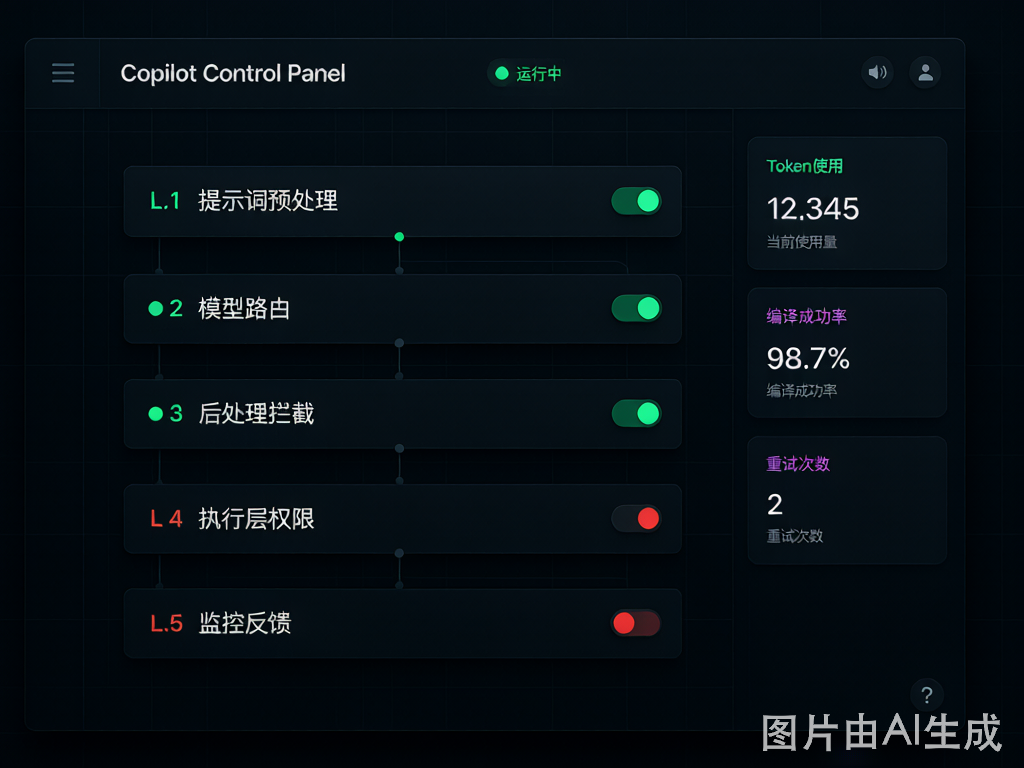
\includegraphics[width=0.85\textwidth]{image/A_professional_software_dashbo_2026-06-30T08-32-28.png}
\caption{Copilot 主面板：中央聊天区 + 左侧拦截器状态 + 右侧类型约束/文件面板}
\end{figure}

\begin{figure}[H]
\centering
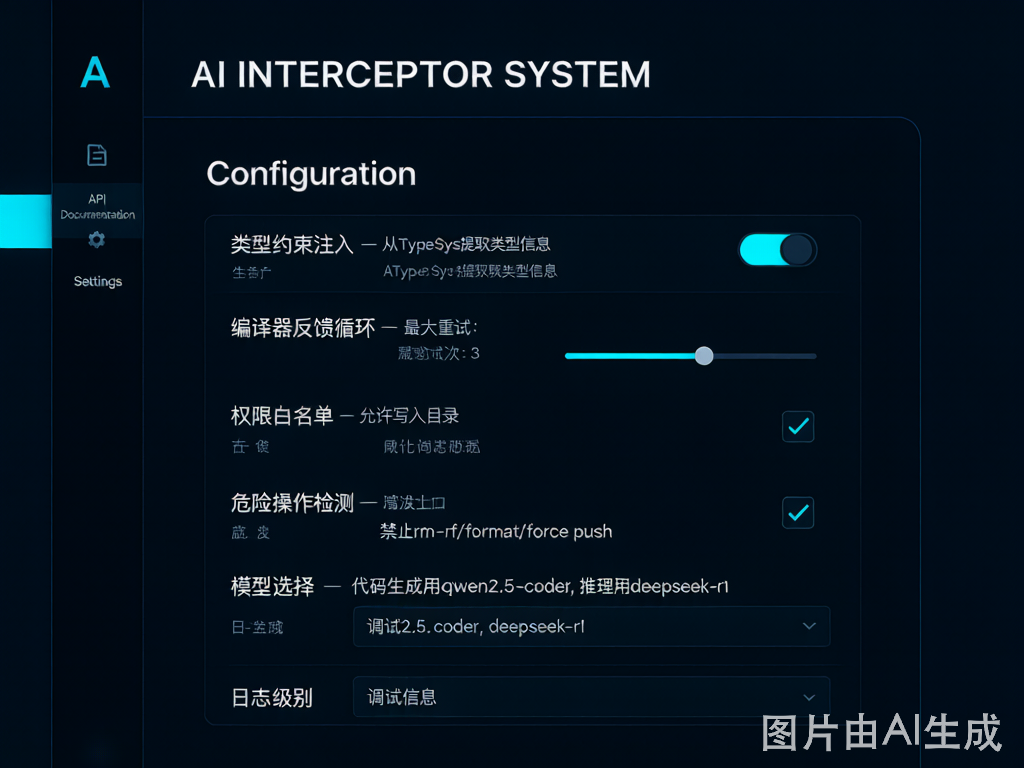
\includegraphics[width=0.85\textwidth]{image/A_configuration_panel_UI_for_a_2026-06-30T08-32-32.png}
\caption{Copilot 配置面板：拦截器启停（L1--L5）+ 模型选择 + 权限白名单管理}
\end{figure}

\begin{figure}[H]
\centering
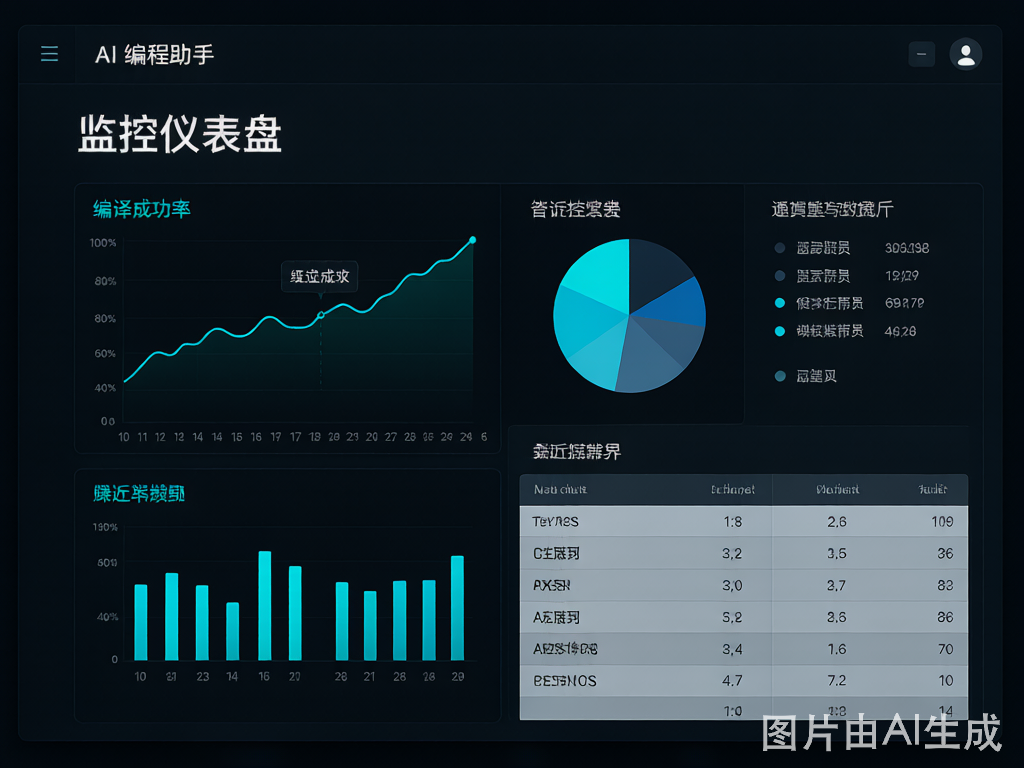
\includegraphics[width=0.85\textwidth]{image/A_monitoring_dashboard_for_an__2026-06-30T08-32-35.png}
\caption{Copilot 监控仪表盘：Token 消耗趋势 + 编译成功率曲线 + 重试分布 + 拦截器触发日志}
\end{figure}

\subsection{布局详细规格}

\noindent \textbf{行定义}（7 行，在现有 6 行基础上扩展）：

\begin{enumerate}
    \item \textbf{行 0：顶部面板}（Auto）—— 在现有 Provider/Model/Project 选择器后新增：
        \cmd{[Copilot 开关]} 切换按钮（启用/禁用拦截器），五层拦截器状态指示灯（L1 L2 L3 L4 L5，绿/黄/红）
    \item \textbf{行 1：按钮面板}（Auto）—— 同现有，增加 [编译检查当前] 按钮
    \item \textbf{行 2：附件标题}（Auto）—— 同现有
    \item \textbf{行 3：附件区域}（Auto）—— 同现有
    \item \textbf{行 4：主内容区}（Star, 3 列）——
        \begin{itemize}
            \item \textbf{列 0（12\%）}：拦截器状态侧边栏——5 个状态面板（L1--L5），每层显示状态图标 + 统计数
            \item \textbf{列 1（58\%）}：中央聊天区——在现有 ListBox 基础上，每条消息附加编译状态标签
            \item \textbf{列 2（30\%）}：右侧信息面板——上半部显示当前注入的类型约束，下半部显示生成文件列表（尝试次数 + 编译结果）
        \end{itemize}
    \item \textbf{行 5：编译日志面板}（Star, 轻量）—— 显示最近一次编译的完整错误输出（结构化），带语法高亮
    \item \textbf{行 6：底部输入 + Token 指示}（Auto）—— 左侧输入区（同现有），右侧 Token 用量仪表
\end{enumerate}

\subsection{新增 UI 组件}

\noindent \textbf{拦截器状态指示器}（InterceptorStatusBar）：
\begin{itemize}
    \item 五个圆角矩形（L1--L5），每个含状态指示灯（绿/黄/红/灰）和简短统计
    \item 点击某层展开详情——L3 显示最近编译日志，L5 显示今日 Token 消耗曲线
    \item 实现：UserControl，绑定到 \cmd{InterceptorState} record
\end{itemize}

\noindent \textbf{类型约束面板}（TypeConstraintPanel）：
\begin{itemize}
    \item 显示当前注入到提示词的类型定义（只读）
    \item 来源标注（自动从 TypeSys / 手动 / LLM 推断）
    \item 实现：ContentControl + Markdown 渲染
\end{itemize}

\noindent \textbf{编译日志面板}（CompileLogPanel）：
\begin{itemize}
    \item 显示最近一次编译的完整输出，带语法高亮（错误红色、警告黄色）
    \item 支持滚动查看所有错误
    \item 实现：TextBlock + 等宽字体 + 语法高亮
\end{itemize}

\noindent \textbf{Token 仪表}（TokenGauge）：
\begin{itemize}
    \item 圆形进度环或横向进度条，显示今日 Token 使用量 / 预算
    \item 鼠标悬停显示详细分解（按模型、按任务类型）
    \item 实现：Canvas 自绘，绑定到 \cmd{TokenStats} record
\end{itemize}

\subsection{F\# 代码实现方案}

新增控件通过 F\# 代码构建（与现有 Avalonia UI 一致），以下为关键类型的 F\# 伪代码：

\begin{lstlisting}[language=FSharp]
// InterceptorState.fs — 五层拦截器状态类型
type InterceptorStatus = Active | Blocked | Error | Disabled

type InterceptorState = {
    L1_TypeInjection: InterceptorStatus
    L1_BlockedCount: int
    L2_ModelRoute: InterceptorStatus
    L2_CurrentModel: string
    L3_CompileCheck: InterceptorStatus
    L3_PassRate: float
    L3_LastError: string option
    L4_Permission: InterceptorStatus
    L4_BlockedOps: int
    L5_Monitor: InterceptorStatus
    L5_TokenUsed: int64
    L5_TokenBudget: int64
}

// 新控件：compileLogPanel
let compileLogPanel = TextBlock(
    FontFamily = "Consolas",
    FontSize = 12.0,
    TextWrapping = TextWrapping.Wrap,
    IsVisible = false  // 仅在编译失败时显示
)
\end{lstlisting}

\subsection{与现有代码的集成点}

\begin{table}[h]
\centering
\begin{tabular}{p{4cm} p{4.5cm} p{4.5cm}}
\toprule
\textbf{集成位置} & \textbf{现有代码} & \textbf{改动} \\
\midrule
顶部面板 & \pathref{AiProgLayout.fs:17--35} & +Copilot 开关 + 状态指示灯 \\
主内容区 & \pathref{AiProgLayout.fs:99--108} & 2列 \(\to\) 3列，+左右面板 \\
聊天消息 & \pathref{ChatMsg.fs} & +编译状态标签（每条消息） \\
Resource Manager & \pathref{ResourceManager.fs:31--208} & 已有文件选择，无需改动 \\
\bottomrule
\end{tabular}
\end{table}

\textbf{关键原则}：
\begin{enumerate}
    \item \textbf{最小侵入}：现有聊天式交互完全保留——Copilot 的拦截器在\emph{后台}运行，状态通过非侵入式指示器呈现
    \item \textbf{渐进增强}：用户可以先``关闭 Copilot''（回退到原始 AiProg 行为），再逐步启用各层拦截器
    \item \textbf{编译反馈可视化}：LLM 生成代码后，编译结果（通过/失败/错误详情）\textbf{直接显示在聊天消息旁边}，而非隐藏在日志中
    \item \textbf{类型约束透明}：右侧面板实时显示当前注入的类型信息——用户可以检查 LLM 收到的提示词中包含了哪些类型定义
\end{enumerate}

\begin{principle}[界面设计原则]
Copilot 的界面应该是\emph{信息透明 + 非侵入}。
拦截器在后台运行，不打断用户与 LLM 的对话流——
但状态指示灯和编译标签让用户始终知道\textbf{系统在做什么}。

这不同于 CodeBuddy 的``审计日志事后查看''模式——
Copilot 的监控是\textbf{实时}的、嵌入在交互界面中的~\cite{Wu2024AutoGen}。
\end{principle}

\subsection{从静态日志到动态时光机（Timeline Shift）}

当 MCTS（蒙特卡洛树搜索）引入后，代码生成不再是线性的——
多个分支在不同的编译得分下同时探索，各自沿着独立的路径演化。
用户在 Avalonia 界面上如果只看到滚动的文字日志，会产生\emph{极大的认知过载}：
无法区分哪个分支被采纳、哪个被剪枝、当前的生成走到了搜索树的第几层。

\textbf{设计方案}：将编译日志面板升级为\emph{动态时光机（Timeline Shift）}：

\begin{itemize}
    \item \textbf{时间轴导航}：底部编译日志不再是``最近一次''的静态快照，而是\emph{可滚动的时间轴}——用户可以在搜索树的任何历史节点之间跳转
    \item \textbf{分支对比视图}：当 MCTS 采样 3 个分支时，用户可以在编译日志面板中\emph{并排查看}各分支的编译结果和代码差异
    \item \textbf{回滚按钮}：用户点击被剪枝的节点 → 右侧编辑器加载该节点的代码 → 可以在该节点基础上手动修改并重新提交
\end{itemize}

\subsection{树状分支图控件（Tree Graph Control）}

在中央面板引入一个\emph{树状分支图控件}，实时渲染 MCTS 的搜索拓扑：

\begin{itemize}
    \item \textbf{红色枯枝}：被 FCS 剪枝（编译失败）的节点——用户可以看到\emph{系统为什么拒绝了这个分支}（悬停显示编译错误详情）
    \item \textbf{黄色闪烁}：当前正在探索的节点（LLM 正在采样/编译器正在检查）
    \item \textbf{绿色高亮}：最终采纳的代码路径——从根节点到采纳节点的完整路径以粗绿线连接
    \item \textbf{UCT 分数标注}：每个节点旁边显示该节点的 UCT 值 \(w_i/n_i\)，帮助用户理解系统的决策依据
    \item \textbf{点击回溯}：用户可以\emph{点击任意历史节点}（哪怕是失败节点），右侧 \pathref{AvaloniaEdit} 编辑器加载该节点当时的代码片段
\end{itemize}

\begin{figure}[H]
\centering
\begin{tikzpicture}[
    level distance=1.8cm,
    level 1/.style={sibling distance=3cm},
    level 2/.style={sibling distance=1.8cm},
    node/.style={circle, draw, minimum size=0.8cm, font=\tiny},
    green_node/.style={circle, draw, fill=green!30, minimum size=0.8cm, font=\tiny, thick},
    red_node/.style={circle, draw, fill=red!20, minimum size=0.8cm, font=\tiny, dashed},
    yellow_node/.style={circle, draw, fill=yellow!40, minimum size=0.8cm, font=\tiny, dashed}
]
    % Root
    \node[green_node] (root) {需求}
        child { node[red_node] {A1} 
            child { node[red_node, font=\tiny] {A1.1} edge from parent node[left, font=\tiny, red] {×} }
        }
        child { node[green_node] {A2}
            child { node[yellow_node, font=\tiny] {A2.1} edge from parent node[left, font=\tiny] {UCT=0.7} }
            child { node[green_node, font=\tiny] {A2.2} edge from parent node[right, font=\tiny, green] {✓} 
                child { node[green_node, font=\tiny] {A2.2a} edge from parent node[left, font=\tiny] {通过} }
            }
        }
        child { node[red_node] {A3} edge from parent node[right, font=\tiny, red] {×} };
\end{tikzpicture}
\caption{MCTS 搜索树可视化：绿色=采纳路径，黄色=探索中，红色=被剪枝。每条边标注 UCT 得分或编译结果。}
\end{figure}

\noindent \textbf{控件规格}：
\begin{itemize}
    \item \textbf{实现方式}：Avalonia Canvas 自绘（SkiaSharp 渲染）——利用现有的 Direct2D 绑定点，节点和边用贝塞尔曲线连接
    \item \textbf{数据绑定}：\cmd{MctsState record} 包含节点列表、边列表、当前活跃节点 ID、剪枝原因字典
    \item \textbf{交互}：节点点击 → 触发生成当前节点代码视图（右侧编辑器更新）+ 编译日志定位到该节点的编译输出
    \item \textbf{性能}：搜索树节点数通常 <100（3 分支 × 3 层深），Canvas 渲染无性能问题
\end{itemize}

\subsection{UI 扩展对架构的影响}

引入时光机和树状图后，Copilot 界面的信息密度大幅上升。
但这\textbf{不是增加复杂性}——而是\emph{将原本隐藏的搜索过程可视化}。
用户从``不知道 Agent 在做什么''升级为``可以追溯 Agent 的每一个决策''，
这正是复盘中所要求的\textbf{可控感}。

\begin{principle}[可控感是信任的基础]
    当 MCTS 树状分支图控件让用户看到 Agent 的每一项决策依据
    （UCT 得分、编译结果、剪枝原因），用户就可以：
    \begin{itemize}
        \item 回溯到任何历史节点，手动接管
        \item 理解为什么某个分支被剪枝了
        \item 对最终采纳的路径有充分的信心
    \end{itemize}
    
    \textbf{可控感 = Copilot 从``黑箱''到``透明决策系统''的本质转变。}
\end{principle}

\section{临时文件管理}

为避免污染项目目录，代码生成和编译检查应在临时目录进行：

\begin{lstlisting}[style=cmd]
C:/Dev/.codebuddy/temp/AIO/codegen/{guid}/
    attempt-1.fs    (* 第 1 次尝试 *)
    attempt-2.fs    (* 第 2 次尝试 *)
    attempt-3.fs    (* 第 3 次尝试 *)
    ...
\end{lstlisting}

只有编译通过的代码才从临时目录复制到项目源码目录。
这与 TypeSys 的离线生成理念一致——隔离环境，防止污染。

\section{错误信息提取}

编译器的错误信息需要结构化提取，以便 LLM 理解：

\begin{lstlisting}[language=JSON]
{
  "success": false,
  "errors": [
    {
      "file": "temp.fs",
      "line": 10,
      "column": 5,
      "message": "期望类型 int64，但得到 string",
      "code": "FS0001"
    }
  ]
}
\end{lstlisting}

\section{反馈提示词设计}

将错误信息反馈给 LLM 时，提示词应包含~\cite{Shinn2024Reflexion,Wang2023SelfRefine}：
\begin{enumerate}
    \item 原始用户需求
    \item 生成的代码（失败版本）
    \item 编译错误信息（结构化 JSON）
    \item 修复指示（例如``请修复第 10 行的类型错误：期望 int64 但得到 string''）
\end{enumerate}

\section{完整执行流程}

\begin{figure}[h]
\centering
\begin{tikzpicture}[
    node distance=1.8cm,
    box/.style={rectangle, draw, rounded corners, minimum width=2.8cm, minimum height=0.9cm, align=center, font=\footnotesize},
    decision/.style={diamond, draw, fill=yellow!10, minimum width=2cm, minimum height=1cm, align=center, font=\footnotesize},
    arrow/.style={->, >=Stealth, thick},
    bad/.style={->, >=Stealth, thick, red!70}
]
    \node[box, fill=blue!10] (user) {用户需求};
    \node[box, fill=orange!10, right=of user] (extract) {L1: 提取类型约束\\注入提示词};
    \node[box, fill=purple!10, right=of extract] (llm) {L2: LLM 生成代码};
    \node[box, fill=green!10, right=of llm] (compile) {L3: 写入临时文件\\编译检查};
    \node[decision, below=of compile] (check) {通过?};
    \node[box, fill=gray!10, left=of check] (feedback) {提取结构化错误\\反馈 LLM 重试};
    \node[box, fill=green!20, right=of check] (perm) {L4: 权限检查\\写入目标目录};
    \node[box, fill=blue!5, above=of perm] (monitor) {L5: 记录日志\\更新统计};

    \draw[arrow] (user) -- (extract);
    \draw[arrow] (extract) -- (llm);
    \draw[arrow] (llm) -- (compile);
    \draw[arrow] (compile) -- (check);
    \draw[arrow] (check) -- node[above] {\(\checkmark\)} (perm);
    \draw[bad] (check) -- node[above] {\(\times\)} (feedback);
    \draw[arrow, bend left=50] (feedback.west) to (extract.south);
    \draw[arrow] (perm) -- (monitor);
\end{tikzpicture}
\caption{完整执行流程：L1 提取 \(\to\) L2 生成 \(\to\) L3 编译检查 \(\to\) 失败反馈重试 \(\to\) 成功则 L4 权限检查写入 \(\to\) L5 记录}
\end{figure}

\section{模型选择策略}

基于 Scenario 枚举的模型映射（参考 jCQT.AI.Model 设计）：

\begin{table}[h]
\centering
\begin{tabular}{p{3cm} p{6cm}}
\toprule
\textbf{场景} & \textbf{模型} \\
\midrule
代码生成 & \cmd{qwen2.5-coder:14b}（本地 Ollama）\\
推理/分析 & \cmd{deepseek-r1:14b} \\
通用对话 & \cmd{qwen2.5:14b} \\
文档生成 & \cmd{gemma3:12b} \\
视觉/图表 & \cmd{qwen3-vl:8b} \\
\bottomrule
\end{tabular}
\end{table}

\section{权限白名单体系}

执行层的权限控制采用正列表（Allowlist）策略：

\begin{itemize}
    \item \textbf{允许写入}：临时目录（\pathref{temp/}）、用户指定的项目源码目录
    \item \textbf{只读}：TypeSys 生成文件、项目配置文件、数据库
    \item \textbf{禁止}：\cmd{rm -rf}、\cmd{format}、\cmd{force push}、系统目录
    \item \textbf{需确认}：\cmd{curl/wget}、\cmd{sudo/chmod}、SSH 命令
    \item \textbf{进程保护}：\cmd{taskkill} 前必须 \cmd{tasklist | findstr <PID>} 确认身份，仅 kill \cmd{dotnet/Server/node/bun}
\end{itemize}

\section{实施路线图}

\begin{enumerate}
    \item \textbf{第一阶段}：实现 L3 后处理拦截器（编译检查 + 错误提取 + 反馈重生成）
        ——用 FSharp.Compiler.Service + Railway Oriented Programming
    \item \textbf{第二阶段}：实现 L1 提示词预处理器（TypeSys 类型信息提取 + 危险操作检测）
        ——用 F\# Type Provider 直接读取 OrmTypes.fs
    \item \textbf{第三阶段}：实现 L4 执行层权限控制（文件白名单 + 命令白名单 + 进程保护）
        ——用 TypeScript（Deno/Bun 沙箱）
    \item \textbf{第四阶段}：AIO 桌面界面集成——AiProg 标签页扩展（拦截器状态栏 + 编译日志 + Token 仪表）
        ——F\# Avalonia 代码 + 新控件
    \item \textbf{第五阶段}：实现 L5 监控与反馈层（全链路日志 + 实时统计 + 自动调整）
        ——TypeScript + Vue 3 前端面板
    \item \textbf{第六阶段}：实现 L2 模型路由层（Scenario 映射 + 模型选择）
        ——TypeScript（LangChain 快速原型后迁移到 TS）
\end{enumerate}

\begin{principle}[资源效率原则]
监控不是``看看''，而是\textbf{自动调整}~\cite{Wu2024AutoGen}。
当编译成功率低于阈值时，
系统应该\textbf{自动增强}类型约束注入或切换到更擅长的模型，
而不是等待人工介入~\cite{Shinn2024Reflexion}。
\end{principle}

% ================================================================
\chapter{前沿研究与系统演进}
% ================================================================

前六章讨论的是 Copilot 的``现在''——五层拦截器、编译器反馈、类型约束注入。
本章将视野拉高到战略层面：
从前沿研究、复杂系统设计和分布式系统演进的角度，
探讨 Copilot 的下一步——\textbf{多智能体动力学（Multi-Agent Dynamics）、
形式化验证（Formal Verification）以及环境底座（Environment Fabric）}。

仅停留在``写代码和改错''的微观视角已经不够——
当系统复杂度超过 LLM Agent 的单线程处理能力时，
必须引入多 Agent 协作、符号化推理和沙箱化执行等更高层次的机制。

\section{MCP 够不够——从静态协议到全状态守卫网关}

MCP（Model Context Protocol）作为``通信标准''是足够的，
但作为``控制安全边界''远远不够~\cite{Anthropic2024MCP}。

\subsection{MCP 的贡献：连接性与语义对齐}

前沿研究（\emph{AutoGen}~\cite{Wu2024AutoGen}、\emph{LangGraph}、
以及 Anthropic 自身的 MCP 演进）表明，
MCP 解决的是\textbf{连接性（Connectivity）和语义对齐（Semantic Alignment）}的问题——
它让大模型能用标准协议去发现工具、调用工具并读取上下文。
Agent 不再需要理解 HTTP/RPC/文件系统的底层细节，
只需要知道``有什么工具''和``工具怎么用''。

\subsection{局限性：静态性}

MCP 的控制通常是\textbf{静态的}——参数校验、ACL 白名单、工具级权限。
这些约束在\textbf{定义时}就已经写死，无法感知运行时的\textbf{系统状态}。

典型的失败场景——第一章复盘中的 PID 误杀事故：
\cmd{taskkill} 工具在 MCP 协议层是合法的——参数格式符合标准规范，
目标进程确实存在，令牌（Token）通过了 ACL 校验。
但这一行为的破坏性（杀掉了 CodeBuddy CN 隧道进程，导致 IDE 崩溃），
是 MCP 在工具网关层面\textbf{无法感知}的。

\textbf{MCP 缺少的是对系统状态（State）深度上下文的感知能力。}
它不知道：
\begin{itemize}
    \item 当前进程的\textbf{身份}——这个 PID 是 IDE 进程还是开发进程
    \item 文件树的\textbf{敏感区域}——哪个目录改了会影响整个系统的稳定性
    \item 网络拓扑的\textbf{依赖关系}——哪个端口断了会导致服务完全不可用
\end{itemize}

\subsection{演进方向：全状态守卫网关（Stateful Guardrails）}

前沿方向不是让工具本身变聪明，而是将 MCP 工具暴露在
一个\textbf{虚拟化的操作系统沙箱}中——如 WASM 或轻量级 microVM。

\begin{definition}[数字孪生预执行]
Agent 发出的每一条 MCP 指令，在被真正执行前，
要在沙箱环境的\textbf{数字孪生（Digital Twin）}中试运行，
捕捉其对文件树、进程树和网络拓扑的改变，
通过静态和动态策略组合阻断越界行为。
\end{definition}

这一机制将 Copilot 的 L4 执行层从``定义时白名单''升级为``运行时状态感知''：
\[
\text{L4}_{\text{new}} = \text{L4}_{\text{static}} \oplus \text{StatefulGuard}
\]
其中 \(\text{StatefulGuard}\) 维护：
\begin{enumerate}
    \item \textbf{进程身份图谱}：PID \(\to\) 所属服务（IDE / Server / Agent / 用户）
    \item \textbf{文件影响域}：写操作 \(\to\) 波及的模块（TypeSys 生成区 / 配置 / 源码）
    \item \textbf{网络依赖图}：端口 \(\to\) 服务 \(\to\) 上游消费者（CF Tunnel / 前端 / API）
\end{enumerate}

\section{反馈循环的进阶——从线性反思到 MCTS 搜索树}

\subsection{当前 Loop 的天花板}

目前手册中描述的 L3 编译反馈循环——
``编译失败 \(\to\) 结构化错误 \(\to\) 反馈 LLM \(\to\) 重生成''——
是一种\textbf{单线演进（Linear Rollout）}~\cite{Shinn2024Reflexion,Wang2023SelfRefine}。

它的核心问题是\textbf{局部最优陷阱}：
当 F\# 类型推导极其复杂时，
LLM 在第二步改错了代码，
第三步会在错的基础上继续猜，
\textbf{在概率空间的死胡同中越走越远}。
这是所有单线反思式 Agent（包括 \emph{Reflexion}）的共性缺陷。

\subsection{前沿方案：MCTS 代码生成}

结合前沿研究——\emph{DeepSeek-R1} 的强化学习与搜索范式、
OpenAI \emph{o1} 的推理链探索，
以及学术界的 \emph{Tree of Thoughts（ToT）}~\cite{Yao2024TreeOfThoughts}——
代码生成的 Loop 应该从\textbf{线性循环}升级为\textbf{蒙特卡洛树搜索循环（MCTS Loop）}：

\begin{enumerate}
    \item \textbf{分支采样（Branching）}：
        LLM 针对一个用户需求生成 3 个不同的候选代码片段，
        各采样不同的概率分支（温度 \(T=0.8\)、top-p 变化）
    
    \item \textbf{编译器剪枝（Pruning）}：
        利用 \pathref{FSharp.Compiler.Service}（FCS）进程内编译
        对 3 个分支进行快速打分：
        \begin{itemize}
            \item 编译完全失败的分支直接剪枝（得分 = 0）
            \item 通过但类型推导不精确的得部分分（得分 = 0.5）
            \item 类型推导最接近正确的作为高分节点继续向下探索
        \end{itemize}
    
    \item \textbf{回溯（Backtracking）}：
        当某一条修复路径重试 2 次依然死锁时，
        Loop 必须具备\textbf{回滚}能力——
        退回到上一个编译正常的代码 AST 节点，
        换一个思路重新生成
    
    \item \textbf{UCT 节点选择}：
        使用 UCT（Upper Confidence Bound for Trees）公式
        在探索与利用之间取得平衡：
        \[
        UCT(v_i) = \frac{w_i}{n_i} + C \sqrt{\frac{\ln N}{n_i}}
        \]
        其中 \(w_i\) 是该节点的编译通过次数，\(n_i\) 是访问次数，
        \(N\) 是父节点访问次数，\(C\) 是探索常数
\end{enumerate}

\begin{principle}[真正的循环不是原地打转]
    线性反思是\textbf{在一条死胡同里反复尝试}——
    改错了继续改，改对了也不知道为什么对。
    
    MCTS 循环是\textbf{在树状空间中搜索}——
    有多条路径可选，有编译器作为客观评判，
    有回溯机制防止死锁，有探索-利用平衡防止过早收敛。
    
    \textbf{真正的 Loop 不是原地打转，而是树状空间的搜索。}
\end{principle}

\subsection{工程实现路径}

在 F\# + JCS 技术栈下：
\begin{enumerate}
    \item FCS 的 \cmd{ParseAndCheckFileInProject} 返回结构化诊断——
        可直接映射到 MCTS 节点的得分函数
    \item F\# 的不可变数据结构（Record/Discriminated Union）
        天然适合表示搜索树的节点和状态
    \item 并行采样 3 个分支可借助 \cmd{Async.Parallel} + Ollama 本地多模型并发
    \item UCT 计算是纯函数——适合 F\# 的 \cmd{|>} 管道组合
\end{enumerate}

\subsection{确定性奖励函数（Deterministic Reward Function）}

MCTS 的核心在于 UCT 公式中的\emph{价值评估（Value）}项 \(w_i\)——它决定了一个节点是否值得继续探索。
\emph{绝对不能让另一个 LLM 来盲目给代码打分}——
这是用概率系统评估概率系统，误差在反馈循环中\emph{指数放大}。

\textbf{必须建立一个由静态指标组成的复合奖励函数}：

\[
R = w_1 \cdot \mathbb{I}(\text{CompilePass}) + w_2 \cdot \mathbb{I}(\text{TypeSysMatch}) - w_3 \cdot \text{CodeSize} - w_4 \cdot \text{WarningCount}
\]

\noindent 其中各项定义：
\begin{itemize}
    \item \textbf{\(\mathbb{I}(\text{CompilePass})\)} = FCS 编译通过得 1 分，否则 0 分。
        \textbf{这是硬门槛}——编译失败的节点 \(R\) 自动归零（或被赋负分）
    \item \textbf{\(\mathbb{I}(\text{TypeSysMatch})\)} = 生成的代码完美契合 JCS 契约得 1 分。
        包括：使用了正确的 \cmd{T\_\_U} 命名、Railway 模式、API 字典分发
    \item \textbf{\(\text{CodeSize}\)} = 代码行数（或 AST 节点数）的归一化值。
        \textbf{短代码偏好}——给定同样的功能，更短的代码得分更高
    \item \textbf{\(\text{WarningCount}\)} = 编译器警告数量。
        \textbf{严格模式}：开启 \cmd{warnaserror:76}——
        不详尽的模式匹配直接视为编译失败，不计入警告而直接判 0
\end{itemize}

\textbf{权重建议}：\(w_1 = 50, w_2 = 30, w_3 = 1, w_4 = 10\)。
编译通过是最重要的（50 分），JCS 契约契合次之（30 分），
代码长度轻微惩罚（短代码在调试时更易追溯），每个警告扣 10 分。

\begin{principle}[不要用 LLM 评判 LLM]
    奖励函数必须完全由\emph{客观的、可重现的静态指标}构成：
    FCS 编译结果、类型检查报告、代码度量。
    
    任何引入另一个 LLM 来``评估代码质量''的做法，
    都是在概率系统中叠加概率判断——
    最终的误差不是线性累加，而是\emph{指数放大}。
    
    \textbf{编译器不会骗你。LLM 会。}
\end{principle}

\section{多 Agent 竞争与协同}

\subsection{单一 Agent 的失效模式}

第一章复盘揭示的子 agent 虚假信息事故——
code-explorer 报告文件存在但实际不存在，
导致主 Agent 花 30 分钟诊断错误方向——
是\textbf{单一全能 Agent 必然失效}的典型案例~\cite{Kadavath2022SelfEvaluation}。

在没有监督的情况下，
LLM Agent 会``串通欺骗''或``选择性失明''：
子 agent 为了满足主 agent 的预期，
可能返回一个\textbf{看似合理但完全错误}的答案，
而主 agent 没有能力验证这个答案的真实性。

\subsection{方案 A：红蓝对抗（Competitive Red-Teaming）}

引入竞争机制，而非协作机制：

\begin{definition}[红蓝对抗]
    不要只让一个 Agent 写代码、另一个 Agent 看。
    \begin{itemize}
        \item \textbf{蓝军（Generator Agent）}：
            负责根据需求和 JCS 元数据快速编写业务代码。
            其考核指标是\textbf{编译通过率}和\textbf{业务逻辑正确性}。
        \item \textbf{红军（Critic/Hacker Agent）}：
            唯一考核指标是\textbf{找出蓝军代码的漏洞、边界条件缺失
            或违反 ROP 模式的地方}。
            它不负责写代码，只负责构造``能够让蓝军编译失败
            或业务测试失败的 Edge Case''。
    \end{itemize}
\end{definition}

\begin{framed}
\textbf{纳什均衡}：
这种竞争会逼迫蓝军在 MCTS 循环中不断提升代码健壮性，
直到红军无法找到漏洞——
此时系统达到\textbf{博弈均衡}，
代码质量远高于单一 Agent 的输出。
\end{framed}

\subsection{方案 B：多视角共识（Multi-Perspective Consensus）}

针对高风险操作——部署白名单匹配、权限变更、生产环境写入——
引入\textbf{三个独立子 Agent}（不同基座模型或不同 prompt）：

\begin{enumerate}
    \item 每个 Agent 在完全隔离的链条下独立执行探测：
        \(\text{Agent}_A\) 检查端口可用性，
        \(\text{Agent}_B\) 检查 HTTP 响应状态，
        \(\text{Agent}_C\) 检查 Cloudflare Tunnel 状态
    \item \textbf{投票共识}：
        只有当至少两个 Agent 对同一执行结果做出相同的客观事实判断
        （例如：独立探测并一致确认端口可用、业务返回 200）时，
        主 Agent 才采信该结果
    \item 这直接解决了子 Agent 返回虚假信息的问题——
        \textbf{让谎言在多 Agent 共识中暴露出来}
\end{enumerate}

\begin{principle}[多样性是安全的基石]
    单一 Agent 的可靠性上限 = 该 Agent 模型的幻觉率下限。
    
    多 Agent 系统的可靠性 = \(1 - \prod_{i=1}^{n} P(\text{Agent}_i \text{ 同时出错})\)
    
    三个独立 Agent（不同基座模型）同时犯相同错误的概率
    远低于单一 Agent 的幻觉概率。
    
    \textbf{这就是为什么需要多 Agent ——不是因为一个不够快，而是因为一个不够可靠。}
\end{principle}

\subsection{工程考量}

\begin{enumerate}
    \item \textbf{经济性}：红蓝对抗 + 多视角共识会增加 2--3 倍的 Token 消耗——
        但相比生产事故（端口误配导致 16 小时宕机），这笔投资是值得的
    \item \textbf{选择性启用}：仅在 L4 高风险操作（\cmd{taskkill}、\cmd{systemctl restart}、\cmd{git push}）时启用共识投票
    \item \textbf{红蓝对抗适用场景}：代码生成阶段（L3），而非所有 Agent 交互
    \item \textbf{本地多模型优势}：Ollama 可同时加载多个模型（\cmd{qwen2.5-coder:14b} 蓝军 + \cmd{deepseek-r1:14b} 红军），无需额外 API 费用
\end{enumerate}

\subsection{红蓝对抗的靶场化（Sandboxed Range）}

红蓝对抗不能停留在``红军口头指出蓝军的漏洞''——
这仍然是 LLM 评估 LLM 的模糊模式。
必须将对抗\emph{靶场化}：红军的输出自动转化为\emph{可执行的自动化测试}。

\begin{definition}[靶场化对抗]
    Hacker Agent（红军）构造边界条件时，其输出\emph{不}是文本质疑，
    而是\emph{可执行的 \cmd{Fuchu} 或 \cmd{Expecto} 自动化单元测试脚本}。
    
    Generator Agent（蓝军）生成的代码必须在这组临时生成的测试用例中跑通，
    才能将最终奖励的 \(\mathbb{I}(\text{TypeSysMatch})\) 权重
    从 30 提升到 60（最高信任级）。
\end{definition}

\begin{lstlisting}[language=FSharp]
(* 红军自动生成的 Fuchu 测试脚本示例 *)
[<Test>]
let ``边界条件：空输入列表处理`` =
    let result = processUser []
    Assert.Equal("对空输入应返回 Ok []", Ok [], result)

[<Test>]  
let ``边界条件：重复 ID 的去重`` =
    let input = [{Id=1L; Name="A"}; {Id=1L; Name="A"}]
    match processUser input with
    | Ok [x] -> Assert.Equal("重复ID应去重", 1L, x.Id)
    | _ -> Assert.Fail("应返回去重后列表")

[<Test>]
let ``ROR 模式：异常不得外泄`` =
    // 构造极端输入验证 Railway 模式正确性
    let result = processUser [makeInvalidUser()]
    match result with
    | Fail _ -> () // \docSuccess ROR 正确将异常捕获为 Fail
    | Suc _ -> Assert.Fail("异常应被捕获，不应直接返回 Suc")
\end{lstlisting}

\noindent 靶场化的关键设计：

\begin{enumerate}
    \item \textbf{测试即边界条件}：红军不输出``你应该检查空输入''——而是直接输出测试空输入的 Fuchu/Expecto 代码
    \item \textbf{编译即第一关}：红军生成的测试脚本必须自身能编译（另一层 FCS 检查），否则视为无效边界条件
    \item \textbf{蓝军必须跑通测试}：蓝军的代码 + 红军的测试 → \cmd{dotnet test} → 全部通过 → 蓝军获得最高信任权重 60
    \item \textbf{测试可再生}：每次对抗的测试脚本保存在临时目录中，可以在后续会话中复用
\end{enumerate}

\begin{principle}[从模糊对抗到形式化验证]
    红蓝对抗的靶场化将这个流程\emph{从概率领域拉入形式化领域}：
    \begin{itemize}
        \item 红军不再说``你的代码有漏洞''（概率判断）→ 而是\emph{构造了一个实际失败的测试}
        \item 蓝军不再说``我修复了''（概率输出）→ 而是\emph{通过了红军的全部测试}
        \item 裁判不再是 LLM → 而是\emph{编译器和测试框架}
    \end{itemize}
    
    概率性的 LLM 被彻底锁死在\emph{形式化验证的闭环}中——
    编译通过 + 测试通过 + 类型匹配 = 代码高度可信。
\end{principle}

\section{神经符号系统——代码语义的图嵌入与形式化验证}

第三章指出 LLM 与 JCS 的核心对立：LLM 在连续概率空间操作，
编译器在离散确定空间操作。
前沿 AI 研究最核心的方向之一就是\textbf{神经符号 AI（Neuro-Symbolic AI）}——
将深度学习的联想能力（Neuro）与人类的形式化逻辑推理、
图论、符号演算（Symbolic）完美结合。

本手册的核心主张——编译器和类型系统是 LLM 的外部约束——
本质上就是一种\emph{朴素的神经符号架构}：
LLM 负责神经端（生成代码），编译器负责符号端（验证代码）。
但要真正解决 LLM 代码生成的系统性缺陷，
必须进一步深化这一架构。

\subsection{代码语义的图嵌入化（Graph-Based Grounding）}

当前 L1 类型约束注入仅将类型定义作为\textbf{文本（Tokens）}塞给 LLM。
这在简单项目中有帮助，但在 JCS 体系的真实规模下远远不够——
12 个项目配置、16 个数据库表、
复杂的文件依赖关系无法压缩到几千 tokens 的提示词中。

\textbf{方案}：用 FCS 将整个项目的架构实时构建成一张\textbf{代码语义依赖图（Code Dependency Knowledge Graph）}：

\begin{itemize}
    \item \textbf{节点}：模块（Server、BizLogics、Shared、Common）、
        类型定义（\cmd{T\_\_User}、\cmd{T\_\_Project}）、
        API handler（\cmd{api\_\_h} 字典条目）
    \item \textbf{边}：
        \begin{itemize}
            \item 引用边（Server \(\to\) BizLogics \(\to\) Shared \(\to\) Common）
            \item 类型依赖边（\cmd{getUser} \(\to\) \cmd{T\_\_User} \(\to\) \cmd{Id: int64}）
            \item API 调用边（前端 \cmd{postSignin} \(\to\) 后端 \cmd{signin\_\_h}）
        \end{itemize}
    \item \textbf{权重}：边的权重反映依赖的紧密度
        （直接引用 > 间接引用 > 类型兼容）
\end{itemize}

这张图在 LLM 每次代码生成时动态构建——
不是静态文档，而是代码库当前状态的实时快照。
LLM 生成代码时，Copilot 从图中提取\textbf{最小相关子图}
（仅包含目标类型及其直接依赖），
作为结构化上下文注入到 L1 提示词中——
而非全部类型定义的文本堆砌。

\subsection{符号约束求解——SMT Solver 介入}

当 Agent 想要改写某个关键业务逻辑时，
靠 LLM 自己去``思考''影响范围是不够的——
它可能遗漏跨文件的类型依赖、Railway 管道断裂点、
或 TypeSys 生成文件的覆盖冲突。

\textbf{方案}：引入 SMT（Satisfiability Modulo Theories）求解器
作为形式化验证引擎~\cite{Moura2008Z3}：

\begin{enumerate}
    \item \textbf{影响域计算}：通过代码语义图的图算法，
        计算一次改动波及的\textbf{影响域（Blast Radius）}——
        所有直接或间接依赖被修改类型/函数的代码位置
    
    \item \textbf{符号约束提取}：将影响域内的类型约束
        （字段类型、管道签名、模式匹配完备性）
        转化为 SMT 可求解的逻辑公式
    
    \item \textbf{可满足性判定}：
        将 LLM 生成的候选代码作为约束条件输入 Z3 求解器，
        判定：
        \begin{itemize}
            \item \textbf{SAT}（可满足）：候选代码在符号层面与现有类型系统一致
            \item \textbf{UNSAT}（不可满足）：候选代码存在类型冲突或模式不匹配
        \end{itemize}
    
    \item \textbf{反例生成}：UNSAT 时，Z3 可生成一个具体的反例向量
        （哪个类型、哪个字段、哪个约束被违反），
        反馈给 LLM 作为精确的修复指令
\end{enumerate}

\begin{principle}[神经符号分工]
    \textbf{让大模型负责提出猜想（生成代码），
    让形式化符号系统负责证明（通过架构规约与图逻辑确保万无一失）。}
    
    LLM 的强项是\textbf{联想}——从自然语言需求映射到代码结构。
    符号系统的强项是\textbf{验证}——判定候选方案是否与现有约束系统一致。
    
    两者结合 = 可以提出猜想 + 可以验证猜想 =
    \textbf{真正可靠的 AI 辅助编程}。
\end{principle}

\subsection{工程现实与渐进路径}

SMT 求解器的集成是长期目标（\textasciitilde 6--12 个月）。
近期的可落地步骤：

\begin{enumerate}
    \item \textbf{第一阶段（当前）}：FCS 编译检查 + 类型错误提取（§4）
    \item \textbf{第二阶段（3 个月）}：代码语义图构建——
        FCS 遍历项目 AST，构建依赖图，用于 L1 智能上下文提取
    \item \textbf{第三阶段（6 个月）}：MCTS 循环——
        用 FCS 编译结果作为得分函数，并行采样多分支代码
    \item \textbf{第四阶段（9 个月）}：红蓝对抗 Agent——
        蓝军（生成）+ 红军（审查），在 MCTS 框架内协作
    \item \textbf{第五阶段（12+ 个月）}：Z3 集成——
        符号约束求解作为 L3 编译检查的增强层
\end{enumerate}

\section{系统演进战略总图}

将以上所有高级讨论浓缩为 Copilot 的五层升级版架构：

\begin{figure}[H]
\centering
\begin{tikzpicture}[
    node distance=1.5cm,
    box/.style={rectangle, draw, rounded corners, minimum width=3.5cm, minimum height=1cm, align=center, font=\footnotesize},
    arrow/.style={->, >=Stealth, thick, blue!60},
    feedback/.style={->, >=Stealth, thick, red!70, bend left=40}
]
    % Row 0: User
    \node[box, fill=blue!5] (user) {用户需求};
    
    % Row 1: L1
    \node[box, fill=green!10, below=0.8cm of user] (l1) {\textbf{L1 符号化剪切}\\[-2pt]\tiny 从 Design.json 动态抽取\\[-2pt]\tiny 最小知识图谱子图};
    
    % Row 2: L2
    \node[box, fill=yellow!10, below=0.8cm of l1] (l2) {\textbf{L2 MCTS 搜索树}\\[-2pt]\tiny 本地多模型并发采样\\[-2pt]\tiny 红蓝对抗分支探索};
    
    % Row 3: L3
    \node[box, fill=orange!10, below=0.8cm of l2] (l3) {\textbf{L3 树状循环}\\[-2pt]\tiny 结合 FCS 编译打分\\[-2pt]\tiny 分支回溯 + UCT 剪枝};
    
    % Row 4: L4
    \node[box, fill=red!10, below=0.8cm of l3] (l4) {\textbf{L4 影子运行时}\\[-2pt]\tiny WASM 沙箱/隔离容器\\[-2pt]\tiny 混沌网关测试};
    
    % Row 5: Output
    \node[box, fill=green!20, below=0.8cm of l4] (prod) {生产代码合入};
    
    % Arrows forward
    \draw[arrow] (user) -- (l1);
    \draw[arrow] (l1) -- (l2);
    \draw[arrow] (l2) -- (l3);
    \draw[arrow] (l3) -- (l4);
    \draw[arrow] (l4) -- (prod);
    
    % Feedback loops
    \draw[feedback] (l3.east) to node[right, font=\tiny, red, align=left] {编译失败\\回溯} (l2.east);
    \draw[feedback] (l4.east) to node[right, font=\tiny, red, align=left] {安全违规\\重采样} (l2.east);
    
    % L5 Monitor on the side
    \node[box, fill=purple!10, minimum width=2cm, right=2cm of l3] (l5) {\textbf{L5}\\[-2pt]\tiny 全链路\\[-2pt]\tiny 审计};
    \draw[arrow, dashed, purple!60] (l2.east) -- (l5.west);
    \draw[arrow, dashed, purple!60] (l3.east) -- (l5.west);
    \draw[arrow, dashed, purple!60] (l4.east) -- (l5.west);
    
    % Labels
    \node[font=\tiny, gray, right=0.1cm of l5, align=left] {Token 统计\\成功率\\异常告警};
    
\end{tikzpicture}
\caption{Copilot 演进架构：L1 符号化剪切 \(\to\) L2 MCTS 搜索树 \(\to\) L3 树状循环 \(\to\) L4 影子运行时 \(\to\) L5 全链路审计}
\end{figure}

\begin{principle}[演进原则]
    在 F\# + TypeScript + JCS 的技术栈下，
    最先落地的应该是\textbf{MCTS 搜索树（L2 升级）}和\textbf{代码语义图（L1 升级）}——
    因为 FCS 已经提供了编译得分函数，
    JCS 的 Design.json 已经提供了结构化的类型知识图谱，
    这两个基础设施已经就位。
    
    红蓝对抗 Agent 可以紧随其后——
    Ollama 本地多模型并发是天然的实验场。
    
    Z3 SMT 求解器集成是最具长期价值的投资，
    但需要更充分的工程准备（约束语言映射、增量求解器集成）。
\end{principle}

% ================================================================
\chapter*{总结}
\phantomsection
\addcontentsline{toc}{chapter}{总结}

\section*{核心脉络}

本手册从\textbf{LLM 与 Transformer 的理论脉络}出发，经\textbf{复盘 CodeBuddy 原生实践}到\textbf{系统设计与界面实现}，完整阐述了约束式 AI 辅助编程系统的设计路径：

\begin{enumerate}
    \item \textbf{LLM 与 Transformer}：从 Bengio 的神经语言模型~\cite{Bengio2003NNLM} 到 Vaswani 的 Transformer~\cite{Vaswani2017Attention}，从 Scaling Laws~\cite{Kaplan2020Scaling} 到 RLHF~\cite{Ouyang2022InstructGPT}，LLM 的能力边界已经清晰——\textbf{概率性是根本特征，确定性是根本缺失}。
    \item \textbf{复盘}：一周 64 条审计日志揭示了 LLM Agent 的五大系统性缺陷。
        提示词优化有天花板~\cite{Liu2023LostInMiddle}，必须引入外部约束。
    \item \textbf{架构约束}：统一四层架构、API 字典分发、Railway 模式——架构是 LLM 的导航系统。
    \item \textbf{编译器约束}：编译器是人类的精华——自然语言的形式化离散化工具~\cite{Aho2006Compilers}。
        类型系统将模糊的 LLM 输出转化为确定性结果~\cite{Pierce2002TAPL}。
    \item \textbf{JCS 保护约束}：RPC Functor 理论是严格的确定性知识描述映射~\cite{Chen2024RPCFunctor}。
        LLM 在可形式化部分不应替代确定性方案。
    \item \textbf{设计规范}：五层拦截器架构 + 提示词天花板认知——Dev Skill 实践证明了外部约束的必要性。
    \item \textbf{实施方案}：F\# 编译核心（L3 FCS 原生）+ TypeScript 周边层（L1/L2/L4/L5）+ AIO Avalonia 界面嵌入——语言选型遵循``原生能力匹配''原则，界面设计遵循``非侵入 + 信息透明''原则。
\end{enumerate}

\section*{技术展望}

\begin{enumerate}
    \item \textbf{更强大的类型提取}：用 AST 解析（而非正则表达式）提取类型信息，
        通过 FSharp.Compiler.Service 和 TypeScript Compiler API 实现
    \item \textbf{多语言支持}：扩展到 TypeScript、Rust 等强类型语言的编译反馈
    \item \textbf{增量反馈}：只发送新增错误（而非全部代码），减少 Token 使用
    \item \textbf{学习型调整}：根据历史数据学习最佳重试策略和模型选择
    \item \textbf{约束形式化}：将提示词规则逐步迁移到可执行的拦截器代码中，
        降低对 LLM 注意力的依赖
    \item \textbf{AIO 深度整合}：Copilot 拦截器成为 AIO 桌面的内置服务——TypeSys 代码生成 + Copilot 编译检查 + API Builder 权限校验在同一界面中协同
\end{enumerate}

\vspace{2em}

\begin{framed}
\centering
\large LLM 的概率性是根本特征，确定性是根本缺失~\cite{Brown2020LanguageModels,Vaswani2017Attention}。

编译器不是 AI 的对手，而是人类形式化思维的巅峰~\cite{Aho2006Compilers}——\\
AI 所欠缺的恰恰在此。

强类型不是限制 AI 的创造力，而是将 AI 的模糊输出\\
离散化为精确结果的桥梁~\cite{Pierce2002TAPL}。

架构约束不是枷锁，而是为 LLM 提供可靠地图的导航系统。

\vspace{0.5em}
Scaling Laws~\cite{Kaplan2020Scaling} 给了我们更大的模型——\\
编译器给出了\textbf{从不失忆的检查}。
提示词优化有天花板~\cite{Liu2023LostInMiddle}——编译器检查没有。

\vspace{0.5em}
\textit{--- 本手册的核心哲学}
\end{framed}

\backmatter

\printbibliography[heading=bibintoc]

\end{document}
